%%%%%%%%%%%%%%%%%%%%%%%%%%%%%%%%%%%%%%%%
% datoteka diploma-FRI-vzorec.tex
%
% vzorčna datoteka za pisanje diplomskega dela v formatu LaTeX
% na UL Fakulteti za računalništvo in informatiko
%
% na osnovi starejših verzij vkup spravil Franc Solina, maj 2021
% prvo verzijo je leta 2010 pripravil Gašper Fijavž
%
% za upravljanje z literaturo ta vezija uporablja BibLaTeX
%
% svetujemo uporabo Overleaf.com - na tej spletni implementaciji LaTeXa ta vzorec zagotovo pravilno deluje
%

\documentclass[a4paper,12pt,openright]{book}
%\usepackage{listings}
%\usepackage{xcolor}
%\lstset { %
%    language=C++,
%    backgroundcolor=\color{black!5}, % set backgroundcolor
%    basicstyle=\footnotesize,% basic font setting
%}
%\documentclass[a4paper, 12pt, openright, draft]{book}  Nalogo preverite tudi z opcijo draft, ki pokaže, katere vrstice so predolge! Pozor, v draft opciji, se slike ne pokažejo!
 
\usepackage[utf8]{inputenc}   % omogoča uporabo slovenskih črk kodiranih v formatu UTF-8
\usepackage[slovene,english]{babel}    % naloži, med drugim, slovenske delilne vzorce
\usepackage[pdftex]{graphicx}  % omogoča vlaganje slik različnih formatov
\usepackage{fancyhdr}          % poskrbi, na primer, za glave strani
\usepackage{amssymb}           % dodatni matematični simboli
\usepackage{amsmath}           % eqref, npr.
\usepackage{hyperxmp}
\usepackage[hyphens]{url}
\usepackage{csquotes}
\usepackage[pdftex, colorlinks=true,
						citecolor=black, filecolor=black, 
						linkcolor=black, urlcolor=black,
						pdfproducer={LaTeX}, pdfcreator={LaTeX}]{hyperref}

\usepackage{color}
\usepackage{soul}
\usepackage[dvipsnames]{xcolor}
\usepackage{dirtree}
\usepackage{minted}
\usepackage{tikz}
\usepackage{siunitx}
\usetikzlibrary{shapes, positioning, matrix}
\usepackage[
backend=biber,
style=numeric,
sorting=nty,
]{biblatex}


\addbibresource{literatura.bib} %Imports bibliography file


%%%%%%%%%%%%%%%%%%%%%%%%%%%%%%%%%%%%%%%%
%	DIPLOMA INFO
%%%%%%%%%%%%%%%%%%%%%%%%%%%%%%%%%%%%%%%%
\newcommand{\ttitle}{Razvoj DBMS jedra z integracijo v programski jezik Python}
\newcommand{\ttitleEn}{Development of a DBMS core with integration into the Python programming language}
\newcommand{\tsubject}{\ttitle}
\newcommand{\tsubjectEn}{\ttitleEn}
\newcommand{\tauthor}{Janez Sedeljšak}
\newcommand{\tkeywords}{Podatkovne baze, C++, Python, B+ drevesa, Podatkovne strukture, SQL, DBMS, ORM}
\newcommand{\tkeywordsEn}{Databases, C++, Python, B+ trees, Data structures, SQL, DBMS, ORM}

%%%%%%%%%%%%%%%%%%%%%%%%%%%%%%%%%%%%%%%%
%	HYPERREF SETUP
%%%%%%%%%%%%%%%%%%%%%%%%%%%%%%%%%%%%%%%%
\hypersetup{pdftitle={\ttitle}}
\hypersetup{pdfsubject=\ttitleEn}
\hypersetup{pdfauthor={\tauthor}}
\hypersetup{pdfkeywords=\tkeywordsEn}

%%%%%%%%%%%%%%%%%%%%%%%%%%%%%%%%%%%%%%%%
% postavitev strani
%%%%%%%%%%%%%%%%%%%%%%%%%%%%%%%%%%%%%%%%  

\addtolength{\marginparwidth}{-20pt} % robovi za tisk
\addtolength{\oddsidemargin}{40pt}
\addtolength{\evensidemargin}{-40pt}

\renewcommand{\baselinestretch}{1.3} % ustrezen razmik med vrsticami
\setlength{\headheight}{15pt}        % potreben prostor na vrhu
\renewcommand{\chaptermark}[1]%
{\markboth{\MakeUppercase{\thechapter.\ #1}}{}} \renewcommand{\sectionmark}[1]%
{\markright{\MakeUppercase{\thesection.\ #1}}} \renewcommand{\headrulewidth}{0.5pt} \renewcommand{\footrulewidth}{0pt}
\fancyhf{}
\fancyhead[LE,RO]{\sl \thepage} 
%\fancyhead[LO]{\sl \rightmark} \fancyhead[RE]{\sl \leftmark}
\fancyhead[RE]{\sc \tauthor}              % dodal Solina
\fancyhead[LO]{\sc Diplomska naloga}     % dodal Solina


\newcommand{\BibLaTeX}{{\sc Bib}\LaTeX}
\newcommand{\BibTeX}{{\sc Bib}\TeX}

%%%%%%%%%%%%%%%%%%%%%%%%%%%%%%%%%%%%%%%%
% naslovi
%%%%%%%%%%%%%%%%%%%%%%%%%%%%%%%%%%%%%%%%  

\newcommand{\autfont}{\Large}
\newcommand{\titfont}{\LARGE\bf}
\newcommand{\clearemptydoublepage}{\newpage{\pagestyle{empty}\cleardoublepage}}
\setcounter{tocdepth}{1}	      % globina kazala

%%%%%%%%%%%%%%%%%%%%%%%%%%%%%%%%%%%%%%%%
% konstrukti
%%%%%%%%%%%%%%%%%%%%%%%%%%%%%%%%%%%%%%%%  
\newtheorem{izrek}{Izrek}[chapter]
\newtheorem{trditev}{Trditev}[izrek]
\newenvironment{dokaz}{\emph{Dokaz.}\ }{\hspace{\fill}{$\Box$}}


%%%%%%%%%%%%%%%%%%%%%%%%%%%%%%%%%%%%%%%%%%%%%%%%%%%%%%%%%%%%%%%%%%%%%%%%%%%%%%%
%% PDF-A
%%%%%%%%%%%%%%%%%%%%%%%%%%%%%%%%%%%%%%%%%%%%%%%%%%%%%%%%%%%%%%%%%%%%%%%%%%%%%%%

%%%%%%%%%%%%%%%%%%%%%%%%%%%%%%%%%%%%%%%% 
% define medatata
%%%%%%%%%%%%%%%%%%%%%%%%%%%%%%%%%%%%%%%% 
\def\Title{\ttitle}
\def\Author{\tauthor, js0578@student.uni-lj.si}
\def\Subject{\ttitleEn}
\def\Keywords{\tkeywordsEn}

%%%%%%%%%%%%%%%%%%%%%%%%%%%%%%%%%%%%%%%% 
% \convertDate converts D:20080419103507+02'00' to 2008-04-19T10:35:07+02:00
%%%%%%%%%%%%%%%%%%%%%%%%%%%%%%%%%%%%%%%% 
\def\convertDate{%
    \getYear
}

{\catcode`\D=12
 \gdef\getYear D:#1#2#3#4{\edef\xYear{#1#2#3#4}\getMonth}
}
\def\getMonth#1#2{\edef\xMonth{#1#2}\getDay}
\def\getDay#1#2{\edef\xDay{#1#2}\getHour}
\def\getHour#1#2{\edef\xHour{#1#2}\getMin}
\def\getMin#1#2{\edef\xMin{#1#2}\getSec}
\def\getSec#1#2{\edef\xSec{#1#2}\getTZh}
\def\getTZh +#1#2{\edef\xTZh{#1#2}\getTZm}
\def\getTZm '#1#2'{%
    \edef\xTZm{#1#2}%
    \edef\convDate{\xYear-\xMonth-\xDay T\xHour:\xMin:\xSec+\xTZh:\xTZm}%
}

%\expandafter\convertDate\pdfcreationdate 

%%%%%%%%%%%%%%%%%%%%%%%%%%%%%%%%%%%%%%%%
% get pdftex version string
%%%%%%%%%%%%%%%%%%%%%%%%%%%%%%%%%%%%%%%% 
\newcount\countA
\countA=\pdftexversion
\advance \countA by -100
\def\pdftexVersionStr{pdfTeX-1.\the\countA.\pdftexrevision}


%%%%%%%%%%%%%%%%%%%%%%%%%%%%%%%%%%%%%%%%
% XMP data
%%%%%%%%%%%%%%%%%%%%%%%%%%%%%%%%%%%%%%%%  
\usepackage{xmpincl}
%\includexmp{pdfa-1b}

%%%%%%%%%%%%%%%%%%%%%%%%%%%%%%%%%%%%%%%%
% pdfInfo
%%%%%%%%%%%%%%%%%%%%%%%%%%%%%%%%%%%%%%%%  
\pdfinfo{%
    /Title    (\ttitle)
    /Author   (\tauthor, js0578@student.uni-lj.si)
    /Subject  (\ttitleEn)
    /Keywords (\tkeywordsEn)
    /ModDate  (\pdfcreationdate)
    /Trapped  /False
}

%%%%%%%%%%%%%%%%%%%%%%%%%%%%%%%%%%%%%%%%
% znaki za copyright stran
%%%%%%%%%%%%%%%%%%%%%%%%%%%%%%%%%%%%%%%%  

\newcommand{\CcImageCc}[1]{%
	\includegraphics[scale=#1]{cc_cc_30.pdf}%
}
\newcommand{\CcImageBy}[1]{%
	\includegraphics[scale=#1]{cc_by_30.pdf}%
}
\newcommand{\CcImageSa}[1]{%
	\includegraphics[scale=#1]{cc_sa_30.pdf}%
}

%%%%%%%%%%%%%%%%%%%%%%%%%%%%%%%%%%%%%%%%%%%%%%%%%%%%%%%%%%%%%%%%%%%%%%%%%%%%%%%
%%%%%%%%%%%%%%%%%%%%%%%%%%%%%%%%%%%%%%%%%%%%%%%%%%%%%%%%%%%%%%%%%%%%%%%%%%%%%%%

\begin{document}
\selectlanguage{slovene}
\frontmatter
\setcounter{page}{1} %
\renewcommand{\thepage}{}       % preprečimo težave s številkami strani v kazalu

%%%%%%%%%%%%%%%%%%%%%%%%%%%%%%%%%%%%%%%%
%naslovnica
 \thispagestyle{empty}%
   \begin{center}
    {\large\sc Univerza v Ljubljani\\%
%      Fakulteta za elektrotehniko\\% za študijski program Multimedija
%      Fakulteta za upravo\\% za študijski program Upravna informatika
      Fakulteta za računalništvo in informatiko\\%
%      Fakulteta za matematiko in fiziko\\% za študijski program Računalništvo in matematika
     }
    \vskip 10em%
    {\autfont \tauthor\par}%
    {\titfont \ttitle \par}%
    {\vskip 3em \textsc{DIPLOMSKO DELO\\[5mm]         % dodal Solina za ostale študijske programe
    VISOKOŠOLSKI STROKOVNI ŠTUDIJSKI PROGRAM\\ PRVE STOPNJE\\ RAČUNALNIŠTVO IN INFORMATIKA}\par}%
%     UNIVERZITETNI  ŠTUDIJSKI PROGRAM\\ PRVE STOPNJE\\ RAČUNALNIŠTVO IN INFORMATIKA}\par}%
%    INTERDISCIPLINARNI UNIVERZITETNI\\ ŠTUDIJSKI PROGRAM PRVE STOPNJE\\ MULTIMEDIJA}\par}%
%    INTERDISCIPLINARNI UNIVERZITETNI\\ ŠTUDIJSKI PROGRAM PRVE STOPNJE\\ UPRAVNA INFORMATIKA}\par}%
%    INTERDISCIPLINARNI UNIVERZITETNI\\ ŠTUDIJSKI PROGRAM PRVE STOPNJE\\ RAČUNALNIŠTVO IN MATEMATIKA}\par}%
    \vfill\null%
% izberite pravi habilitacijski naziv mentorja!
    {\large \textsc{Mentor}: doc. dr. Boštjan Slivnik\par}%
    {\vskip 2em \large Ljubljana, \the\year \par}%
\end{center}
% prazna stran
%\clearemptydoublepage      
% izjava o licencah itd. se izpiše na hrbtni strani naslovnice

%%%%%%%%%%%%%%%%%%%%%%%%%%%%%%%%%%%%%%%%
%copyright stran
%%%%%%%%%%%%%%%%%%%%%%%%%%%%%%%%%%%%%%%%
\newpage
\thispagestyle{empty}

\vspace*{5cm}
{\small \noindent
To delo je ponujeno pod licenco \textit{Creative Commons Priznanje avtorstva-Deljenje pod enakimi pogoji 2.5 Slovenija} (ali novej\v so razli\v cico).
To pomeni, da se tako besedilo, slike, grafi in druge sestavine dela kot tudi rezultati diplomskega dela lahko prosto distribuirajo,
reproducirajo, uporabljajo, priobčujejo javnosti in predelujejo, pod pogojem, da se jasno in vidno navede avtorja in naslov tega
dela in da se v primeru spremembe, preoblikovanja ali uporabe tega dela v svojem delu, lahko distribuira predelava le pod
licenco, ki je enaka tej.
Podrobnosti licence so dostopne na spletni strani \href{http://creativecommons.si}{creativecommons.si} ali na Inštitutu za
intelektualno lastnino, Streliška 1, 1000 Ljubljana.

\vspace*{1cm}
\begin{center}% 0.66 / 0.89 = 0.741573033707865
%{ \CcImageCc{0.741573033707865}\hspace*{1ex}\CcImageBy{1}\hspace*{1ex}\CcImageSa{1}% }%
\end{center}
}

\vspace*{1cm}
{\small \noindent
Izvorna koda diplomskega dela, njeni rezultati in v ta namen razvita programska oprema je ponujena pod licenco GNU General Public License,
različica 3 (ali novejša). To pomeni, da se lahko prosto distribuira in/ali predeluje pod njenimi pogoji.
Podrobnosti licence so dostopne na spletni strani \url{http://www.gnu.org/licenses/}.
}

\vfill
\begin{center} 
\ \\ \vfill
{\em
Besedilo je oblikovano z urejevalnikom besedil \LaTeX.}
\end{center}

% prazna stran
\clearemptydoublepage

%%%%%%%%%%%%%%%%%%%%%%%%%%%%%%%%%%%%%%%%
% stran 3 med uvodnimi listi
\thispagestyle{empty}
\
\vfill

\bigskip
\noindent\textbf{Kandidat:} Janez Sedeljšak\\
\noindent\textbf{Naslov:} \ttitle \\
\noindent\textbf{Vrsta naloge:} Diplomska naloga na visokošolskem programu prve stopnje Računalništvo in informatika \\
\noindent\textbf{Mentor:} doc. dr. Boštjan Slivnik\\

\bigskip
\noindent\textbf{Opis:}\\
Besedilo teme diplomskega dela študent prepiše iz študijskega informacijskega sistema, kamor ga je vnesel mentor. 
V nekaj stavkih bo opisal, kaj pričakuje od kandidatovega diplomskega dela. 
Kaj so cilji, kakšne metode naj uporabi, morda bo zapisal tudi ključno literaturo.

\bigskip
\noindent\textbf{Title:} \ttitleEn

\bigskip
\noindent\textbf{Description:}\\
opis diplome v angleščini

\vfill



\vspace{2cm}

% prazna stran
\clearemptydoublepage

% zahvala
%\thispagestyle{empty}\mbox{}\vfill\null\it%
%\noindent
%Na tem mestu zapišite, komu se zahvaljujete za pomoč pri izdelavi diplomske naloge oziroma pri vašem študiju %nasploh. Pazite, da ne boste koga pozabili. Utegnil vam bo zameriti. Temu se da izogniti tako, da celotno %zahvalo izpustite.
%$\rm\normalfont

% prazna stran
\clearemptydoublepage

%%%%%%%%%%%%%%%%%%%%%%%%%%%%%%%%%%%%%%%%
% posvetilo, če sama zahvala ne zadošča :-)
%\thispagestyle{empty}\mbox{}{\vskip0.20\textheight}\mbox{}\hfill\begin{minipage}{0.55\textwidth}%
%Svoji dragi Alenčici.
%\normalfont\end{minipage}

% prazna stran
\clearemptydoublepage


%%%%%%%%%%%%%%%%%%%%%%%%%%%%%%%%%%%%%%%%
% kazalo
\setcounter{tocdepth}{2}
\pagestyle{empty}
\def\thepage{}% preprečimo težave s številkami strani v kazalu
\tableofcontents{}


% prazna stran
\clearemptydoublepage

%%%%%%%%%%%%%%%%%%%%%%%%%%%%%%%%%%%%%%%%
% seznam kratic

\chapter*{Seznam uporabljenih kratic}

\noindent\begin{tabular}{p{0.14\textwidth}|p{.4\textwidth}|p{.4\textwidth}}
  {\bf kratica} & {\bf angleško}                              & {\bf slovensko} \\ \hline
  {\bf API} & application programming interface & aplikacijski programski vmesnik \\
  {\bf CI/CD} & continuous integration, continuous delivery & neprekinjena integracija in postavitev \\
  {\bf CLI} & command line interface & vmesnik za ukazno vrstico \\
  {\bf CRUD} & create, read, update, delete & ustvarjanje, branje, posodabljanje in brisanje \\
  {\bf CSV} & comma-separated values & vrednosti, ločene z vejico \\
  {\bf DBMS} & database management system & sistem za upravljanje podatkovnih baz \\
  {\bf ER} & entitiy relationship (diagram) & (diagram) entitet in relaciji \\
  {\bf HTTP} & hypertext transfer protocol & protokol za prenos hiperteksta \\
  {\bf I/O} & input/output operations & vhodno/izhodne operacije \\
  {\bf JSON} & JavaScript object notation & objektna notacija za JavaScript \\
  {\bf NoSQL} & nonrelational databases & nerelacijske podatkovne baze \\
  {\bf ORM} & object-relational mapping & objektno relacijska preslikava \\
  {\bf SQL} & structured query language & strukturiran jezik poizvedb \\
  {\bf TCP/IP} & Internet protocol, transmission control protocol & internetni protokol in protokol za nadzor prenosa \\
\end{tabular}


% prazna stran
\clearemptydoublepage

%%%%%%%%%%%%%%%%%%%%%%%%%%%%%%%%%%%%%%%%
% povzetek
\phantomsection
\addcontentsline{toc}{chapter}{Povzetek}
\chapter*{Povzetek}

\noindent\textbf{Naslov:} \ttitle
\bigskip

\noindent\textbf{Avtor:} \tauthor
\bigskip

%\noindent\textbf{Povzetek:} 
\noindent V diplomskem delu je predstavljenih trenutno nekaj najbolj uporabljenih sistemov za upravljanje podatkovnih baz (DBMS). V veliki meri so standard podatkovnih baz še vedno relacijske podatkovne baze. V ta namen je tekom dela predstavljen razvoj lastnega DBMS za programski jezik Python.

Sam razvoj namenske knjižnice je pripravljen v programskem jeziku C++, saj gre za nizko nivojski jezik, kjer imamo visoko fleksibilnost pri upravljanju s pomnilniku. Predstavljen je razvoj vseh potrebnih segmentov za dobro delujočo relacijsko podatkovno bazo. Ključnega pomena tekom razvoja je bila uporaba dobrih podatkovnih struktur in algoritmov, ki dobro izkoristijo I/O operacije, ki jih ponuja operacijski sistem in posledično pripeljejo do zanesljivega in optimalnega delovanja DBMS.

V zadnjem sklopu diplomskega dela smo pripravili analizo uspešnosti implementacije DBMS na različnih scenarijih, kjer razvito programsko opremo primerjamo z že obstoječima DBMS – SQLite in MySQL.
\bigskip

\noindent\textbf{Ključne besede:} \tkeywords.
% prazna stran
\clearemptydoublepage

%%%%%%%%%%%%%%%%%%%%%%%%%%%%%%%%%%%%%%%%
% abstract
\phantomsection
\selectlanguage{english}
\addcontentsline{toc}{chapter}{Abstract}
\chapter*{Abstract}

\noindent\textbf{Title:} \ttitleEn
\bigskip

\noindent\textbf{Author:} \tauthor
\bigskip

%\noindent\textbf{Abstract:} 
\noindent The thesis presents an overview of some of the currently most widely used Database Management Systems (DBMS). Relational databases still largely dominate the landscape of database standards. With this in mind, the thesis focuses on developing a custom DBMS for the Python programming language.

The development of this dedicated library is carried out in the C++ programming language, chosen for its low-level nature, providing high flexibility in memory management. The development encompasses all necessary components for a well-functioning relational database. Throughout the development process, a crucial aspect has been the utilization of efficient data structures and algorithms, optimizing I/O operations provided by the operating system, resulting in a reliable and optimized DBMS performance.

In the final part of the thesis, a performance analysis of the implemented DBMS is conducted across various scenarios. The developed software is compared against existing DBMS solutions – SQLite and MySQL.
\bigskip

\noindent\textbf{Keywords:} \tkeywordsEn.
\selectlanguage{slovene}
% prazna stran
\clearemptydoublepage

%%%%%%%%%%%%%%%%%%%%%%%%%%%%%%%%%%%%%%%%
\mainmatter
\setcounter{page}{1}
\pagestyle{fancy}

% združimo uvod in kaj so relacijske podatkovne baze
% 1. začnemo z brez podatkovnih baz dan danes negre (gre za trajen način shranjevanja podatkov itd.)
% 2. različni tipi podatkovnih baz
% 2.1 relacijske
% 2.2 nosql
% 3. relacijske in depth

\chapter{Uvod}
    Živimo v dobi, kjer se spopadamo z izzivom obdelave izjemnih količin podatkov, ki jih poznamo kot velike podatke (velepodatki) in predstavljajo dragocen vir informacij. Ko razmišljamo o dolgoročnem shranjevanju teh podatkov, se osredotočamo na uporabo podatkovnih baz. Na tem področju prepoznavamo dve osnovni skupini – relacijske in nerelacijske podatkovne baze.
    \section{Paradigme v svetu podatkovnih baz}
        \subsection{Relacijske podatkovne baze}
        Trenutno na trgu še vedno prevladujejo relacijske podatkovne baze, ki predstavljajo standardno izbiro. Te baze temeljijo na striktni strukturi entitet, kjer so podatki organizirani v smiselne entitete, ki vključujejo stolpce (atribute) in vrstice (zapise). Posebej pomembne so logične povezave med posameznimi zapisi, ki omogočajo boljšo organizacijo in interpretacijo podatkov. Te povezave so realizirane s pomočjo tujih ključev, kar omogoča vzpostavitev trdnih relacij med različnimi entitetami.

        \subsubsection{Kaj je DBMS in kakšna je njegova vloga v bazi podatkov?}

        Kaj hitro, ko začnemo raziskovati interno delovanje relacijskih podatkovnih baz naletimo na pojem DBMS (sistem za uporabljanje podatkovnih baz). Gre za programsko rešitev, ki je zasnovana za upravljanje in organiziranje podatkov. Uporabnikom omogoča ustvarjanje, spreminjanje in poizvedovanje po bazi podatkov \cite{DBMS_G4G}.

        Ko govorimo specifično o relacijskih podatkovnih bazah, pa lahko uporabimo tudi kratico RDBMS (relacijski sistem za uporabljanje podatkovnih baz). 

        \subsubsection{Začetki relacijskih podatkovnih baz}
        Gre za paradigmo podatkovnih baz, ki se je prvič pojavila leta 1970, ko je model za shranjevanje predstavil Edgar F. Codd – matematik izobražen na univerzi Oxford \cite{IBM_DBMS_1970}. Prva družina relacijskih podatkovnih baz, pa je bila razvita leta 1983 – Db2 \cite{DB2}, katero je izdal IBM. Tekom let je Db2 doživel, kar nekaj posodobitev - zadnja med njimi je bila leta 2022, ko je DBMS v svoje delovanje dodal še nekaj konceptov iz umetne inteligence za boljšo izrabo virov \cite{DB213}. Kljub temu je DBMS konceptualno ostal nespremenjen in še vedno uporablja zasnovo relacijskega modela.
        
        \subsection{Nerelacijske podatkovne baze}
        Nerelacijske podatkovne baze predstavljajo novo kategorijo baz, ki temeljijo na bistveno drugačnih osnovah kot tradicionalne relacijske podatkovne baze. Te nove baze so se razvile kot odziv na izzive, s katerimi se srečujejo relacijske podatkovne baze. Glavna ovira relacijskih podatkovnih baz izvira iz njihove stroge strukture. V novi kategoriji podatkovnih baz, znanih kot NoSQL, je ključna lastnost prilagodljivost. Sama organizacija podatkov se bistveno razlikuje, pri čemer tradicionalne entitete in relacije med zapisi nadomeščajo objekti in koncept dedovanja. Ta pristop prinaša tudi eno od glavnih prednosti, ki jih imajo nerelacijske podatkovne baze – sposobnost enkapsulacije posameznih zapisov, ki omogoča učinkovito razporeditev celotne baze na več strežnikov (horizontalno skaliranje podatkov), ki ga tradicionalne relacijske podatkovne baze težje dosežejo.
    
    \section{Kje se danes uporabljajo relacijske podatkovne baze?}

    Relacijske podatkovne baze so že desetletja temeljna komponenta informacijskih sistemov in njihova uporaba se je v današnjem sodobnem poslovnem okolju še povečala. Kljub pojavu novejših tehnologij in podatkovnih modelov imajo relacijske podatkovne baze številne aplikacije, kjer izstopajo zaradi svoje strukture, zanesljivosti in možnosti za kompleksno analizo.

    \subsection{Vloga DBMS v informacijskih sistemih}

    Na sliki \ref{infsistem} je predstavljena standardna zasnova arhitekture za večino modernih informacijskih sistemov:
    \begin{figure}[h]
        \centerline{\includegraphics[height=0.5\textwidth, angle=0]{webarchitecture.png}}
        \caption{Struktura sodobnega informacijskega sistema}
        \label{infsistem}
    \end{figure}

    \noindent
    Diagram je sestavljen iz treh ključnih komponent. Na eni strani so odjemalci, ki vključujejo mobilne, spletne aplikacije  ... Ti odjemalci s strežniškim delom aplikacije komunicirajo preko standardiziranih HTTP metod na nivoju povezovalne API komponente.

    Večji del informacijskega sistema, pa se nahaja v uporabniku skritem delu, kjer je realizirana poslovna logika in upravljanje s podatki oz. bazo podatkov. V sodobnih informacijskih sistemih za dodaten nivo varnosti in lažjo manipulacijo podatkov pogosto uporabimo še ORM (objektno relacijska preslikava). Gre za kos programske opreme, ki omogoča lažjo delo s podatkovno bazo. Entitete znotraj ORM se preslikajo v razrede, zapisi znotraj entitete, pa so predstavljeni kot instance teh razredov. ORM predstavlja dodaten nivo abstrakcije, ki programerju med drugim omogoči tudi avtomatske migracije podatkovne baze, kot tudi lažjo integracijo podatkovne baze znotraj uporabljenega programskega jezika.

    \section{Motivacija za razvoj lastnega DBMS in ORM vmesnika}
    Glavna motivacija za razvoj lastnega DBMS izhaja iz želje po boljšem razumevanju notranjega delovanja podatkovnih baz, ter njihovega vpliva na delovanje modernih aplikaciji. Kot programerji se pogosto osredotočamo le na izgradnjo funkcionalnosti, pri čemer podatkovno bazo pogosto spregledamo oz. spregledamo vpliv le-te na delovanje celotne aplikacije.
    
    Podatkovna baza s seboj prinese visoko raven abstrakcije, ki je podprta z obsežno množico algoritmov in konceptov, ki omogočijo zanesljivo, hitro in varno izvajanje operaciji nad podatki. Tekom razvoja je cilj spoznati tudi te koncepte, ki sicer ostajajo skriti v abstrakciji, ki jo prinašata DBMS in jezik SQL, ki programerju predstavlja način komuniciranja z bazo podatkov.

    Pomembnost podatkovnega sloja, ki vključuje podatkovno bazo, kot tudi del aplikacije, ki je odgovorna za delo s podatki postane očitna, predvsem ko se aplikacija začne odzivati počasneje. Pogost razlog je obsežna količina podatkov v posamezni entiteti, kar za uporabnika hitro pomeni nesprejemljiv čas odzivnosti celotnega sistema.

    Pri iskanju pristopov za optimizacijo podatkovnega sloja hitro naletimo na koncept indeksiranja podatkov. Ta pristop ni omejen zgolj na relacijske podatkovne baze, temveč se pojavlja širom računalniške znanosti. Osnovna ideja za optimizacijo je ustvarjanje iskalne strukture, ki omogoča izrazito hitrejše iskanje podatkov z izrabo učinkovite podatkovne strukture.
    
    Dve bolj pogosti podatkovni strukturi za izvedbo indeksiranja sta zgoščevalne tabele in drevesa. Na področju relacijskih podatkovnih baz se najpogosteje uporablja več nivojsko indeksiranje, ki je realizirano prav z drevesi (v večini primerov gre za B drevo). B drevo je tip drevesa, ki je sestavljeno iz vozlišč, kjer ima vsako največ $M$ zapisov in $M+1$ kazalcev na nadaljnja vozlišča. S pomočjo dodajanja indeksov lahko linearno iskanje, ki ima časovno kompleksnost $O(N)$, kjer je $N$ število vseh zapisov bistveno pohitrimo. Z uporabo B drevesa, namreč dosežemo časovno kompleksnost $O(log_M(N))$, kjer je $N$ število vseh zapisov v drevesu.
    \newline
    \newline
    \noindent
    Pomembno je poudariti, da cilj implementacije lastne rešitve ne vključuje razvoja kompleksnega in dovršenega DBMS, ki bi se primerjal z naprednimi in vzpostavljenimi rešitvami. Naš cilj je razviti knjižnico, ki bo vsebovala temeljne funkcionalnosti in bo primerna za uporabo v manjših aplikacijah. Osredotočili se bomo predvsem na izgradnjo preprostega in intuitivnega načina za upravljanje s podatki.

\chapter{Sorodna dela}

    Prve podatkovne baze so se razvile že pred več kot štiridesetimi leti in ob tem tudi ogromno različnih pristopov za komunikacijo med programskimi jeziki in DBMS. V računalništvu je izbor orodja ključnega pomena in izbor tehnologij znotraj podatkovnega sloja nikakor ne predstavlja izjeme.

    \section{Izbor DBMS}
    Pri izbiri DBMS se soočimo z različnimi možnostmi, med katerimi izstopajo DBMS-ji, kot so Db2 \cite{DB2}, Oracle \cite{ORACLE}, ter Microsoft SQL Server (MSSQL) \cite{MSSQL}, ki predstavljajo največje in najbolj skalabilne DBMS-je. Kljub temu je izbor DBMS-ja, podobno kot pri večini področij v računalništvu, odvisen od zahtev naše aplikacije in narave podatkov, ki jih bomo shranjevali.

    Za mnoge primere morda zadostujeta bolj preprosta DBMS-ja, kot sta PostgreSQL \cite{POSTGRESQL} in MySQL \cite{MYSQL}, ki ponujata enostavno upravljanje in predstavljata dobro izbiro tudi za shranjevanje obsežnih količin podatkov. 
    
    V določenih scenarijih, ko imamo opravka z bolj preprosto in manj obsežno strukturo podatkov (npr. pri razvoju mobilnih aplikaciji), se za najprimernejšo izbiro izkaže SQLite \cite{SQLITE}. Gre za minimalističen DBMS, ki za razliko od prej omenjenih izbir za potrebe shranjevanja podatkov uporablja zgolj datoteko, ki jo zlahka enkapsuliramo v izolirano okolje, kot je mobilna naprava. V področje manjših podatkovnih baz, pa lahko uvrstimo tudi razvit DBMS – Graphenix \cite{GRAPHENIX_GITHUB}.
    
    \section{Statističen pregled Python ORM knjižnic}

    V spodnji tabeli je predstavljena kratka statistična analiza najpogosteje uporabljenih ORM knjižnic, ki so na voljo v programskem jeziku Python. Podatke za število mesečnih in tedenskih prenosov smo pridobili iz spletne platforme PYPI Stats \cite{pypistats}, kjer se nahaja sledenje prenosov posameznih paketov znotraj Python ekosistema. Podatki za število GitHub zvezd, pa so pridobljeni direktno iz repositorijev posameznih knjižnic, ki so dostopne na GitHub platformi.
    
    \noindent
    \begin{center}
        \begin{tabular}{p{0.28\textwidth}|p{.17\textwidth}|p{.18\textwidth}|p{.18\textwidth}}
          {\bf Knjižnica} & {\bf GitHub zvezde} & {\bf Mesečni prenosi} & {\bf Tedenski prenosi} \\ \hline
          {\bf Django \cite{DJANGO_GITHUB}} & \textbf{\num{72} tisoč} & \num{10} milijonov & \num{2,4} milijona \\
          {\bf SQLAlchemy \cite{SQLALCHEMY_GITHUB}} & \num{7,5} tisoč &  \textbf{\num{83} miljonov} & \textbf{\num{20} miljonov} \\
          {\bf Peewee \cite{PEEWEE_GITHUB}} & \num{10} tisoč & \num{1,1} milijon & \num{281} tisoč \\
          {\bf Tortoise ORM \cite{TORTOISE_GITHUB}} & \num{3,7} tisoč & \num{88} tisoč & \num{22} tisoč \\
          {\bf SQLObject \cite{SQLOBJECT_GITHUB}} & 133 & \num{27} tisoč & \num{6} tisoč \\
        \end{tabular}
    \end{center}

    \noindent
    Glede na zgornjo tabelo izluščimo, da v ekosistemu prevladujejo naslednje tri ORM knjižnice:
    \begin{itemize}
        \item \textbf{Django ORM \cite{DJANGO_GITHUB}} je vgrajen del širše Django knjižnice, ki je namenjena izdelavi spletnih aplikaciji. Omogoča zelo širok nabor operaciji nad podatkovno bazo, poleg tega ima vgrajen tudi svoj CLI (vmesnik za ukazno vrstico). S tem celotno ogrodje bistveno pospeši produktivnost razvijalcev, a hkrati kot ogrodje doda, kar 8.9 MB dodatne teže. Knjižnica podpira pet DBMS-jev, to so PostgreSQL \cite{POSTGRESQL}, MariaDB \cite{MARIADB}, MySQL \cite{MYSQL}, Oracle \cite{ORACLE} in SQLite \cite{SQLITE}. Pomembno je izpostaviti, da je število prenosov nekoliko zavajajoče, saj uporaba Django knjižnice v primerih, ko ne potrebujemo trajnega shranjevanja podatkov ne pomeni uporabe Django ORM.
        \item \textbf{SQLalchemy \cite{SQLALCHEMY_GITHUB}} gre za eno najbolj fleksibilnih in uporabljenih knjižnic znotraj programskega jezika. Sama fleksibilnost pomeni, da številne operacije, ki so znotraj Django ORM že avtomatizirane so tukaj prepuščene implementaciji razvijalca. Fleksibilnost, pa s seboj prinaša tudi bistveno prednost, saj lahko kot razvijalec, ki dobro pozna ozadje delovanja uporabljenega DBMS izkoristimo različne pristope optimizaciji, ki jih znotraj Django ORM ni mogoče realizirati oz. je implementacija bistveno težja. Knjižnica zaradi lahkotne abstrakcije podpira SQLite \cite{SQLITE}, MySQL \cite{MYSQL}, Oracle \cite{ORACLE}, MSSQL \cite{MSSQL} in še mnogo drugih DBMS-jev.
        \item \textbf{Peewee \cite{PEEWEE_GITHUB}} je ena izmed preprostejših knjižnic, ki predstavlja lahkoten nivo abstrakcije. Knjižnica podpira 3 relacijske podatkovne baze, to so PostgreSQL \cite{POSTGRESQL}, MySQL \cite{MYSQL} in SQLite \cite{SQLITE}. Gre za dokaj omejen nabor, saj je knjižnica dokaj minimalistična in s seboj ne prinese kompleksnosti, kot to storita Django ORM in SQLalchemy.
    \end{itemize}

    \noindent
    Cilj vseh teh knjižnic je pospešiti proces razvoja aplikacij in zagotoviti dodatno varnost pri delu s podatkovno bazo. Omeniti velja, da te knjižnice omogočajo tudi druge koristne funkcionalnosti, kot je lažja manipulacija s podatki, poenostavljeno vzdrževanje in enostavna migracija strukture. S svojo abstrakcijo in intuitivnimi vmesniki odpravljajo potrebo po neposrednem rokovanju z zapletenimi SQL poizvedbami ter s tem razbremenjujejo razvijalce in omogočajo hitrejši razvoj aplikacij.

    \subsection{Slabost uporabe ORM knjižnic na nivoju poizvedb}
    Kljub vsem dobrim lastnostim omenjenih knjižnic, pa tudi vsaka izmed njih prinaša dodaten nivo abstrakcije in razvijalcu skrije veliko možnosti za optimizacijo delovanja DBMS. V algoritmih je pogost kompromis med hitrostjo in porabo prostora, ko pa govorimo o ORM knjižnicah in programskih jezikih, pa višji nivo abstrakcije pomeni kompromis hitrosti delovanja.

    Narava relacijskih podatkovnih baz in združevanja tabel je usmerjena v skupen rezultat v obliki ene matrike, kjer imamo kartezičen produkt zapisov različnih entitet, katerega filtriramo glede na relacije, ki so realizirane s pomočjo tujih ključev.
    
    Kot ciljni uporabniki pogosto želimo drugačno strukturo, ki pa ni v skladu z osnovno idejo relacijskih baz. V ta namen ORM knjižnice izvedejo več različnih poizvedb in potem znotraj jedra knjižnice združujejo zapise in kreirajo ciljno strukturo ali pa izvedejo eno kompleksnejšo poizvedbo in pridobljene podatke nato preoblikujejo v končno strukturo.
    
    Za primer lahko vzamemo naslednjo nalogo: ``Za vse uporabnike pridobi njihova opravila in sporočila``. Za nalogo je SQLAlchemy \cite{SQLALCHEMY_GITHUB} izvedel naslednjo SQL poizvedbo:
    \begin{minted}{sql}
SELECT * FROM users
LEFT OUTER JOIN tasks AS t ON users.id = t.user_id
LEFT OUTER JOIN messages AS m ON users.id = m.user_id
    \end{minted}

    \noindent
    Zgornji pristop pomeni, da za vsakega uporabnika prenesemo $\max(T_i, 1) \cdot \max(M_i, 1)$ zapisov, kjer je $T_i$ število opravil $i$-tega uporabnika in $M_i$ število sporočil $i$-tega uporabnika. $N$ pa določa skupno število uporabnikov.

    Končno število zapisov, ki jih pridobimo lahko izračunamo s pomočjo vsote ~\eqref{data_sum_first}.
    
    \begin{equation}
        \sum_{i=1}^{N} \max(T_i, 1) \cdot \max(M_i, 1)
    \label{data_sum_first}
    \end{equation}

    \noindent
    Skupno število zapisov, kjer bi vsak zapis iz posamezne entitete pridobili le 1x, pa lahko napišemo kot vsoto ~\eqref{data_sum_second}.

    \begin{equation}
        N + \sum_{i=1}^{N} (T_i + M_i)
    \label{data_sum_second}
    \end{equation}

    \noindent
    Torej najprej potrebujemo $N$ zapisov za vsakega uporabnika, nato pa za vsakega uporabnika pridobimo še $T_i$ opravil in $M_i$ sporočil.
    
    Če predpostavimo, da imamo podatkovno bazo, kjer imamo \num{100} uporabnikov in ima vsak izmed njih \num{1000} sporočil, ter \num{200} opravil pomeni, da bomo v primeru prve vsote~\eqref{data_sum_first} prenesli, kar $(100 \cdot 1000 \cdot 200) = \num{20000000}$ zapisov.

    Medtem, ko v primeru druge vsote~\eqref{data_sum_second} to pomeni prenos bistveno manjše količine podatkov ($(100 \cdot (1000 + 200)) = \num{120000}$. Kar predstavlja le $0.6\%$ podatkov v primerjavi s prvo vsoto.

    Ozko grlo, pa se pojavi še v enem segmentu, namreč pripravljanje končne strukture, ki jo vrne ORM je v vseh treh omenjenih knjižnicah izvedeno na nivoju programskega jezika Python, ki sam po sebi ni optimiziran za filtriranje in združevanje zapisov oz. ne omogoča pristopov, ki jih lahko uporabimo znotraj prevedenih jezikov in tako bistveno pohitrimo kreiranje končne strukture.

\chapter{Razvoj jedra DBMS}
\label{ch0}
    V poglavju predstavimo razvoj jedra DBMS s pomočjo programskega jezika C++. V prvi fazi je predstavljena celotna struktura podatkov in način shranjevanja na disk. Za tem predstavimo razvoj B+ drevesne strukture za optimalno indeksiranje podatkov. Nato se spustimo v predstavitev optimizaciji oz. algoritmov, ki omogočajo hitrejše branje podatkov in za zaključek še predstavitev funkcionalnosti, ki jih naš DBMS podpira.
    \newline
    \newline
    \noindent
    Vsa izvorna koda je dostopna na GitHub repozitoriju \cite{GRAPHENIX_GITHUB}.

    \newpage
    \noindent
    Skozi poglavje bodo vsi primeri dela z DBMS na nivoju programskega jezika Python uporabljali preprost ER model z uporabniki, nalogami in sporočili. Uporabnik lahko ima več nalog in sporočil – pri sporočilih, pa imamo še dodatno vlogo, saj je lahko uporabnik pošiljatelj/prejemnik.
\begin{minted}{python}
import graphenix as gx

class User(gx.Model):
    name = gx.Field.String()
    tasks = gx.Field.VirtualLink("user")
    sent_msgs = gx.Field.VirtualLink("sender")
    recieved_msgs = gx.Field.VirtualLink("reciever")

class Task(gx.Model):
    content = gx.Field.String(size=100)
    user = gx.Field.Link("User").as_index()

class Message(gx.Model):
    content = gx.Field.String(size=50)
    date = gx.Field.DateTime()
    sender = gx.Field.Link("User")
    reciever = gx.Field.Link("User")
\end{minted}
    
    \section{Struktura shranjevanja podatkov}
        \subsection{Datotečna struktura za shranjevanje podatkov znotraj entitet}
        Za vsako posamezno entiteto se privzeto kreirata 2 datoteki $ix\_<naziv\_entitete>.bin$ in $<naziv\_entitete>.bin$.
        \begin{enumerate}
            \item $<naziv\_entitete>.bin$ (matrika podatkov) – je matrična struktura, ki predstavlja dejanske zapise podatkov. Vsaka vrstica predstavlja en zapis, kjer je dolžina vrstice vsota dolžin vseh atributov, ki se shranjujejo v entiteti. Posamezen stolpec matrike predstavlja posamezne atribute v matriki.
            \item $ix\_<naziv\_entitete>.bin$ (glava entitete s kazalci) – gre za vektorsko strukturo, kjer vsaka zaporedna vrstica vsebuje kazalec na dejanski zapis v matriki podatkov – ta kazalec je realiziran, kot celoštevilski odmik zapisa v matriki. Poleg kazalcev struktura vsebuje tudi kazalec na prvo prosto vrstico v matriki:
            \begin{itemize}
                \item Matrika je polna – kazalec na konec datoteke
                \item V matriki podatkov obstaja fragmentacija – kazalec na prvo prosto vrstico v matriki 
            \end{itemize}
        \end{enumerate}

        \begin{figure}[h]
            \centerline{\includegraphics[width=0.7\textwidth, angle=0]{struktura_entitet.png}}
            \caption{Struktura podatkovne matrike in glave entitete s kazalci}
            \label{sl:mindmap}
        \end{figure}

        \colorbox{BurntOrange}{Popravi sliko - izvedba v tikz Latex}
        
        
        \subsection{Tipi podatkov}
        Znotraj razvitega DBMS podpiramo 7 podatkovnih tipov:
        \begin{enumerate}
            \item Cela števila (ang. Int) – v tem primeru gre za vrednost, ki je na nivoju C++ programskega jezika shranjena kot int64\_t oziroma predznačeno celo število. Velikost za posamezno vrednost je 8B. Sam razpon vrednosti, ki jih lahko shranimo v posamezen zapis je $[-2^{63}, 2^{63} - 1]$.
            \item Realna števila (ang. Float) – zaradi lažje implementacije je velikost realnih števil enaka, kot velikost celih števil – torej 64 bitov. Vrednost je na nivoju podatkov realizirana, kot ``dvojni float`` oz. ``double``. Gre za zaporedje bitov, ki so po standardu IEEE 754 \cite{kahan1996ieee} ločeni v predznak, eksponent in mantiso.
            \item Nizi (ang. String) – Gre za zaporedje znakov, kjer na nivoju posamezne entitete določimo maksimalno dovoljeno dolžino posameznega zapisa. Torej velikost posameznega zapisa je $N * 1B$, kjer je $N$ maksimalna dolžina podatka. 
            \item Logične vrednosti (ang. Bool) – je najmanjši podatkovni tip, ki ga vsebuje naš DBMS in zavzame vsega 1B; drži pa lahko vrednosti $0/1$ oz. True/False, kot je to definirano v programskem jeziku Python.
            \item Datumi (ang. Datetime) – gre za podatkovni tip, ki je ponovno shranjen, kot vrednost int64\_t in je predstavljen v EPOCH formatu \cite{EPOCH_FORMAT} – gre za časovni odmik trenutnega časa od UTC datuma 1. 1. 1970. 
            \item Povezava (ang. Link) – gre za vgrajen tip relacije, kjer je podatek kazalec na drug zapis v določeni entiteti. V ozadju je to le primarni ključ določenega zapisa, ki se nastavi avtomatsko (ponovno gre za podatek, ki je zapisan kot int64\_t vrednost).
            \item Virtualna povezava (ang. VirtualLink) – gre za navidezno polje v entiteti, ki ne zavzame nobenega dodatnega prostora. Polje je pomembno za kreiranje povezave ob poizvedbah, kjer na določen zapis vežemo seznam zapisov iz druge tabele.  
        \end{enumerate}
        
        \subsection{Realizacija relaciji med entitetami}

        Implementacija relacij med entitetami se izvaja s pomočjo uporabe tujih ključev, ki predstavljajo primarne ključe identificiranih zapisov in omogočajo povezavo med entitetami. Ti tujih ključi se shranijo kot atributi v entiteto, ki vzpostavlja povezavo, in kažejo na primarni ključ v povezani entiteti. Vzpostavitev povezave se izvede pri ustvarjanju modela na ravni programskega jezika Python.

        Spodaj je predstavljen tudi preprost primer, kjer neko sporočilo vežemo na dva uporabnika, ki imata vlogo pošiljatelja in prejemnika:
\begin{minted}{python}
john = User(name='John Doe').make()
jane = User(name='Jane Doe').make()

first_mesage = Message(
    content = 'Moje prvo sporočilo',
    date = datetime.now(),
    sender = john
    reciever = jane
).make()
\end{minted}

    \section{Indeksiranje z uporabo B+ dreves}
        \subsection{B+ drevesa in njihove značilnosti}

        B+ drevesa so podatkovna struktura, uporabljena za učinkovito indeksiranje in iskanje podatkov.
        Vsako vozišče ima lahko največ $M$ podatkov in $M+1$ kazalcev na nova vozlišča.

        V B+ drevesih so vsi nivoji razen listov drevesa, vmesna vozlišča, ki vsebujejo kazalce na nadaljnja vozlišča znotraj drevesa – služijo le kot povezave ter omogočajo učinkovitejše iskanje in navigacijo po strukturi. Medtem so podatki shranjeni v listih drevesa.

        Definicija strukture zahtevna tudi striktno uravnoteženost drevesa, torej da so vsi listi drevesa na istem nivoju.

        Kot dodatna optimizacija za iskanje intervalov znotraj drevesa je v naši implementaciji dodana še struktura dvojno povezanega seznama na nivoju listov drevesa. Tako ima vsak list kazalec na predhoden in naslednji list v drevesu. Na primeru podatkovne baze, je to zelo uporabno, ko iščemo npr. prvih petdeset uporabnikov razvrščenih po priimku. V prvi fazi je seveda potrebno imeti kreirano indeksno strukturo za iskan atribut. Zatem pa je iskanje zapisov dokaj trivialno, namreč sprehodimo se le do najbolj levega lista v drevesu, nato pa se sprehodimo po povezanem seznamu od leve proti desni in shranimo kazalce na želene zapise, jih nato le preberemo iz matrike podatkov, ter razvrstimo po ciljnem atributu.

        Na sliki \ref{btree_example} je prikazan preprost primer B+ drevesa realiziran s stopnjo $M=2$:
        \colorbox{BurntOrange}{Dodaj še kazalce iz posameznega zapisa v listu (slika)}
        
        \begin{figure}[h]
        
\begin{center}
\begin{tikzpicture}
\tikzstyle{bplus}=[rectangle split,rectangle split horizontal, rectangle split parts = 3, rectangle split empty part width=0.01mm, rectangle split every empty part={\hspace{0.25cm}}, draw]
\tikzstyle{every node}=[bplus]
\tikzstyle{level 1}=[sibling distance=60mm]
\tikzstyle{level 2}=[sibling distance=25mm]
\node {19\nodepart{two}} [->]
child {node {5\nodepart{two}11}
child {node (A) {2\nodepart{two}3}}
child {node (B) {5\nodepart{two}7}}
child {node (C) {11\nodepart{two}17}}
}
child {node {29\nodepart{two}}
child {node (D) {19\nodepart{two}23}}
child {node (E){29\nodepart{two}31}}
}
;
\draw [->] (A) -- (B);
\draw [<-] (A) -- (B);
\draw [->] (B) -- (C);
\draw [<-] (B) -- (C);
\draw [->] (C) -- (D);
\draw [<-] (C) -- (D);
\draw [->] (D) -- (E);
\draw [<-] (D) -- (E);


\end{tikzpicture}
\end{center}

            \caption{Primer B+ drevesa, kjer indeksiramo pošiljatelje sporočil}
            \label{btree_example}
        \end{figure}

        

        \newpage
        \subsection{Pravila, ki jih zahteva B+ drevesna struktura}
        \begin{enumerate}
            \item Vsako vozlišče ima največ $M$ podatkov in $M+1$ kazalcev – kapaciteta vozlišča.
            \item Listi drevesa so vsi na enakem nivoju.
            \item Urejenost – vse vrednosti, ki se nahajajo levo morajo biti manjše ali enake trenutni; vse vrednosti desno, pa marajo biti večje ali enake.
            \item Vozlišče je veljavno, kadar ima vsaj $M/2$ zapisov, kjer je $M$ kapaciteta oz. maksimalno število podatkov, ki jih lahko ima vozlišče.
        \end{enumerate}

        \subsection{Implementacija iskanja v MySQL in SQLite DBMS}
        \colorbox{BurntOrange}{https://dev.mysql.com/doc/refman/8.0/en/index-btree-hash.html}

        \subsection{Implementacija B+ dreves za shranjevanje na disk}
        Zakaj se na področju podatkovnih baz uporabljajo B drevesa. Ozadje je dokaj preprosto, saj klasične iskalne strukture s pomočjo dreves, ki so realizirane s pomočjo binarnih dreves vsebujejo izrazito ozko grlo. Ozko grlo je pride do izraza, ko je drevo shranjeno na disku in potrebujemo za vsako vozlišče izvesti eno branje iz diska.

        Ko beremo vozlišča pomeni eno branje vozlišča en dostop do diska in v primeru binarnega drevesa to pomeni, da je število dostopov do datoteke enako številu podatkov, ki smo jih prebrali - branje vsekakor predstavlja počasno operacijo in število teh branj želimo čim bolj minimizirati.

        B drevesa ta problem rešujejo s samo količino podatkov, ki je shranjena na nivoju enega vozlišča. V klasičnih trdih diskih je velikost enega vozlišča drevesa bila določena, kot velikost sektorja na trdem disku. To je pomenilo, da je branje vsakega vozlišča predstavljalo točno eno branje iz diska.

        Klasičen način določanja velikosti posameznih vozlišč se je dokaj spremenil odkar so standard za shranjevanje podatkov postali hitrejši tipi diskov kot so SSD.
        
        \subsection{Uporaba B+ dreves v bazi podatkov (iskanje po indeksiranih podatkih)}
        Na nivoju podatkovne baze se B+ drevesa uporabljajo za indeksiranje podatkov oz. zapisov glede na določen atribut npr. datum rojstva, ime, hišno številko itd. Gre za pristop, ki nam omogoča filtriranje posameznih zapisov s pomočjo binarnega iskanja v logaritmičnem času namesto linearnega iskanja skozi celotno matriko.
        
        Določanje indeksov, pa je v klasičnih podatkovnih bazah lahko tudi malo bolj kompleksno, saj poleg iskanja po določenem atributu lahko iščemo tudi po izpeljanih vrednostih npr. po kombinaciji prve črke priimka in imena. V primeru našega DBMS to ni realizirano, lahko pa si sami kreiramo dodaten atribut na nivoju entitete in vanj shranjujemo želeno vrednost, ter nato direktno nad atributom kreiramo indeksno strukturo.
        
        \subsection{Dinamično nalaganje in ohranjanje posameznih segmentov drevesa v pomnilnik}
        Za dodatno optimizacijo delovanja internih indeksov je dodana tudi implementacija predpomnilnika, kamor lahko shranjujemo posamezne segmente drevesa. Deluje, kot preprost zgoščevalni slovar, kjer je ključ odmik posameznega vozlišča v fizični datoteki vrednost, pa je dejansko vozlišče.

        Omenjena implementacija nam omogoča preprosto upravljanje z vozlišči, saj je dostop do vsakega vozlišča omogočen preko skupnega vmesnika, ki sicer pomeni dodatno rabo pomnilnika vendar, pa bistveno dvigne varnost, ko želimo opravljati s posameznim zapisom.
        
        \subsection{Slabosti uporabe indeksov}

        Sama raba indeksov je koristna, saj bistveno pohitri postopek iskanja posameznih zapisov glede na določen atribut. Ko govorimo v časovni zahtevnosti to pomeni pohitritev iz $O(N)$ na $O(log_M(N))$.

        Na drugi strani pa se skriva kar nekaj lastnosti B+ dreves, ki jih moramo imeti v mislih ob dodajanju nepotrebnih indeksov v našo podatkovno bazo.
        \begin{itemize}
            \item Časovna zahtevnost vnašanja in posodabljanja zapisov v posamezni entiteti se zaradi vnašanja v B drevo z osnovo $M$ poveča iz $O(1)$ na $O(log_M(N) * X)$, kjer je $X$ število stolpcev z dodano indeksno strukturo. $N$ pa predstavlja število že obstoječih zapisov v posamezni entiteti.
            \item Za vsak postavljen indeks se bistveno poveča poraba prostora na disku, saj shranjevanje drevesne strukture s seboj prinese podvajanje atributa, kot tudi dodatek kazalca na glavo entitete.
        \end{itemize}

        \subsection{Ostali pristopi indeksiranja podatkov}
        \colorbox{BurntOrange}{Indeksiranje s pomočjo zgoščevalnih tabel ...}

    \newpage
    \section{Pomembni gradniki za optimalno izvedbo poizvedb}
        
        \subsection{Gručanje podatkov ob branju iz diska}
        
        Kot je bilo že omenjeno v prejšnjih poglavjih je največje ozko grlo, s katerim se srečujemo I/O operacije (torej pisanje in branje iz/na disk). V ta namen je tudi v segmentu prenosa podatkov iz datoteke v pomnilnik realizirano s čim manj dostopi do diska. V ta namen je ob prvi fazi nabora dodan algoritem za gručenje podatkov.

        Sam problem je zelo preprost imamo urejen vektor celih števil, kjer želimo vrednosti grupirati glede na posamezne odmike in najti skupine oz. gruče in te združiti v eno branje matrične datoteke s podatki. Za primer lahko vzamemo naslednji vektor odmikov v matrični datoteki:

\hfill \break
\begin{figure}[h]
\begin{center}
\begin{tikzpicture}[->, >=stealth, auto]
  % Define the vector elements
  \def\vectorElements{{0, 64, 72, 256, 512, 528, 542, 1024}}
  
  % Set the node style
  \tikzset{listnode/.style={circle, draw, minimum size=1.3cm}}
  
  % Draw the linked list nodes
  \foreach \i/\element in {0/0,1/64,2/72,3/256,4/512,5/528,6/534,7/1024}{
    \node[listnode] (\i) at (\i*1.5,0) {\element};
  }
  
  % Connect the linked list nodes
  \foreach \i [evaluate=\i as \j using {int(\i+1)}] in {0,...,6}{
    \draw (\i) -- (\j);
  }
\end{tikzpicture}
\caption{Zaporedje odmikov za poizvedbo iz matrične datoteke}
\end{center}
\end{figure}

\noindent Iz odmikov lahko hitro razberemo dve gruči, kateri bi želeli, da naš algoritem odkrije in branje nad odmikoma izvede v enem branju - to sta gruči $[64, 62]$, ter $[512, 528, 540]$. Optimalen pristop branja bi lahko barvno označili po naslednji konfiguraciji:

\hfill \break
\begin{figure}[H]
\begin{center}
\begin{tikzpicture}[->, >=stealth, auto]
  \def\vectorElements{{0, 64, 72, 256, 512, 528, 542, 1024}}
  
  \node[circle, draw, minimum size=1.3cm] (0) at (0,0) {0};
  \node[circle, draw, fill=orange!30, minimum size=1.3cm] (1) at (1.5,0) {64};
  \node[circle, draw, fill=orange!30, minimum size=1.3cm] (2) at (3,0) {72};
  \node[circle, draw, fill=gray!30, minimum size=1.3cm] (3) at (4.5,0) {256};
  \node[circle, draw, minimum size=1.3cm, fill=red!30] (4) at (6,0) {512};
  \node[circle, draw, minimum size=1.3cm, fill=red!30] (5) at (7.5,0) {528};
  \node[circle, draw, minimum size=1.3cm, fill=red!30] (6) at (9,0) {534};
  \node[circle, draw, minimum size=1.3cm, fill=black!30] (7) at (10.5,0) {1024};

  \draw (0) -- (1);
  \draw (1) -- (2);
  \draw (2) -- (3);
  \draw (3) -- (4);
  \draw (4) -- (5);
  \draw (5) -- (6);
  \draw (6) -- (7);
\end{tikzpicture}
\caption{Zaporedje odmikov za poizvedbo iz matrične datoteke z obarvanjem gruč}
\end{center}
\end{figure}
        
        \subsubsection{Linearna izvedba gručenja nad urejenim seznamom}
        Za izvedbo gručenja obstaja veliko algoritmov, ki nalogo opravijo zelo dobro vendar s seboj prinesejo visoko časovno zahtevnost. V naši izvedbi gručenja smo želeli poiskati algoritem, kjer gručenje opravimo v linearnem času, saj ob testiranju ostalih algoritmov v večini primerov samo gručenje traja dlje, kot pa branje posameznih elementov v matriki. V ta namen smo pripravili preprost algoritem, ki se sprehodi skozi seznam in spremlja odmike, ter združuje elemente v kolikor ne presežemo zgornje meje velikosti ene gruče in poleg tega zadovoljimo minimalno velikost za gručo.
        
        \subsection{Uporaba prioritetne vrste za urejanje zapisov}

        Ob implementaciji omejevanja števila rezultatov s pomočjo ukazov `limit` in `offset` moramo poskrbeti za časovno optimalno izvedbo poizvedbe, saj iz vidika uporabnika DBMS pričakujemo, da z dodatkom ukaza `limit` čas izvajanja skrajša.

        Tekom razvoja smo testirali nekaj različnih pristopov in podatkovnih struktur. Naš problem lahko definiramo, kot iskanje $K$ najmanjših elementov, kjer je $K$ sestavljen iz dveh komponent $L$ in $O$, kjer je $L$ maksimalno število elementov oz. limita, $O$ pa predstavlja odmik oz. število zapisov, ki jih želimo preskočiti.

        Tekom razvoja smo preizkusili 3 različne pristope za iskanje $K$ najmanjših elementov v seznamu.

        \begin{enumerate}
            \item Klasično vstavljanje v seznam in ureditev elementov ob koncu vnašanja, ter rezanje elementov od indeksa $O$, do vključno $O+L$. Časovna zahtevnost tega pristopa je $O(N \cdot log_2(N))$, prostorska zahtevnost, pa je tukaj $O(N)$, saj moramo v pomnilniku držati vse potencialne elemente.
            \item Postopno vstavljanje v urejen seznam, v tem primeru uporabimo vgrajeno std::vector \cite{CPP_VECTOR} strukturo, kjer vstavljanje izvajamo s pomočjo binarnega iskanja. Težava pristopa se skriva v vstavljanju v začetni del seznama, saj moramo potem vse elemente zamikati za eno mesto v desno. Posledično, čeprav je časovna zahtevnost binarnega iskanja $O(log_2(N))$ zaradi premikanja elementov časovna zahtevnost postane $O(N)$. Tako je časovna zahtevnost celotnega postopka vstavljanja $O(N^2)$ v najboljšem primeru pa $O(N \cdot log_2(K))$. Glavna prednost algoritma pred pristopom urejanja na koncu se nahaja v prostorski zahtevnosti. Ta je namreč le $O(K)$, saj v pomnilniku ohranjamo maksimalno $K$ vrstic in jih po potrebi zamenjujemo ob iteraciji skozi vrstice matrike.
            \item Za daleč najboljši pristop se je izkazalo vstavljanje v prioritetno vrsto, ki je realizirana, kot kopica. Za podatkovno strukturo uporabimo vgrajeno C++ std::priority\_queue \cite{CPP_PQUEUE}. V tem primeru je časovna zahtevnost posameznega vstavljanja $O(log_2(K))$, kar pomeni za $N$ vstavljanj $O(N \cdot log_2(K))$. Prostorska zahtevnost, pa je enako kot v zgornjem primeru $O(K)$. Problem je zastavljen, tako da $K$ ne more nikoli biti večji od $N$ in je posledično časovna zahtevnost tega pristopa najbolj optimalna. Pomemben segment pri uporabi vgrajene prioritetne vrste je tudi izbor podatkovne strukture, ki jo vrsta uporablja za shranjevanje podatkov. Za najbolj optimalen pristop se je izkazal vgrajeni std::vector \cite{CPP_VECTOR}, ki je na nivoju pomnilnika shranjen v enem kosu, kar omogoči prevajalniku in procesorju, da izrabita še optimizacijo z lokalnostjo.
        \end{enumerate}

        \noindent
        Za zgornje tri pristope obstaja veliko spremenljivk, ki vplivajo na čas izvajanja samega algoritma za iskanje $K$ najmanjših elementov v seznamu. Največ vpliva ima vrednost $N$, ki predstavlja število zapisov, ki jih moramo preveriti in primerjati z ostalimi elementi. Je tudi spodnja meja za vse časovne zahtevnosti, vse imajo namreč časovno zahtevnost vsaj $O(N)$. Bistveno bolj zanimiv, pa je vpliv vrednosti $K$, ki predstavlja tudi razliko v časovnih zahtevnostih med posameznimi algoritmi. Za lažje razumevanje, kako vrednost $K$ vpliva na čas izvajanja smo pripravili tudi grafično analizo, kjer v izoliranem okolju izvedemo vse tri algoritme. Vrednost $N$ je nastavljena na $\num{10000000}$, $K$ pa se spreminja na $x$ osi in je definiran na intervalu $[500, 25000]$.

        \begin{figure}[H]
            \centerline{\includegraphics[height=0.52\textwidth, angle=0]{prvih_k_elementov.png}}
            \caption{Časovna primerjava pristopov za iskanje $K$ najmanjših elementov v seznamu.}
            \label{sl:k_smallest}
        \end{figure}

        \noindent
        Iz zgornjega grafa lahko razberemo, da vrednost $K$ nima bistvenega vpliva na prvi in tretji algoritem. Izjema je drugi algoritem, kateri ima sicer časovno zahtevnost $O(N^2)$, vendar je $K$ zelo pomemben faktor, saj večji kot je $K$ večkrat moramo izvesti vstavljanje v vektor, kar pa postaja sorazmerno počasneje glede na večanje vrednosti $K$.

        Izkaže se, da je algoritem z uporabo prioritetne vrste najbolj optimalen pristop, kar pokažejo tudi perfomančni testi, ki se izvajajo na platformi GitHub, saj smo z uporabo omenjenega pristopa dobili do 4x pohitritev izvedbe nabora podatkov iz ene entitete.

        \subsection{Uporaba podatkovnih okvirjev ob poizvedovanju podatkov}

        Akcija za poizvedovanje ob prvi implementaciji deluje po naslednjih korakih:
        \begin{enumerate}
            \item Izgradnja strukture, ki definira vse potrebne parametre za poizvedbo – QueryObject.
            \item Izvedba branja na nivoju programskega jezika C++ in pretvorba zapisov v seznam, kjer je posamezen zapis predstavljen kot slovar.
            \item Pretvorba posameznega slovarja (vrstice) v instanco objekta.
        \end{enumerate}

        \noindent
        Ob profiliranju akcije za poizvedovanje podatkov opazimo, da velik delež izvajalnega časa vzame 3. točka – torej pretvorba posameznega zapisa v instanco razreda.

        Za hitrejšo izvedbo smo na nivoju programskega jezika Python pripravili podatkovno strukturo – pogled (ang. View). Ta struktura omogoča preprečevanje potrebe po tretjem koraku in tudi spreminja predstavitev posameznih vrstic iz strukture slovarja v terko (ang. Tuple). View, pa predstavlja ovoj, ki deluje na podobnem principu, kot delujejo podatkovni okvirji (ang. DataFrame) v knjižnici za podatkovno analitiko \cite{PANDAS_GITHUB}. Struktura smo implementirali na nivoju programskega jezika C++, kar še dodatno pospeši čas dostopa do posameznega zapisa.

        \subsubsection{Optimizacija v številkah}
        Za izmeritev učinkovitosti implementacije, smo uporabili scenarij iz performančnih testov celotnega sistema (branje milijona vrstic in shranjevanje celotnega seznama v pomnilnik).
        \begin{itemize}
            \item V prvi implementaciji je povprečni čas izvajanja bil nekje $\approx 7$ sekund, kjer je več kot 80\% časa predstavljalo instanciranje objektov.
            \item Po optimizaciji, pa celoten čas branja zahteva povprečno $\approx 1.3$ sekunde. Kar v podanem scenariju pomeni, kar 5x pohitritev izvedbe branja.
        \end{itemize}

    \section{Podprte funkcionalnosti na nivoju vgrajenega ORM sistema}
    \begin{itemize}
        \item \textbf{Filtriranje podatkov – funkcija ``filter`` (DBMS – where).}
        \newline
        \noindent
        Parametri te funkcije se drevo, kjer je posamezno vozlišče drevesa predstavljeno z enim ali več pogoji, ki so oviti v AND ali OR pogoj.
        
        Vozlišče v katerem želimo, da vsi pogoji držijo kreiramo s pomočjo ``gx.every(...)`` metode, medtem ko za kreiranje vozlišča z vezavo ali uporabimo metodo ``gx.some(...)``.
        
\begin{minted}[breaklines]{Python}
john = User(name='John Doe').make()
jane = User(name='Jane Doe').make()
...
query = Message.filter(
    Message.date.greater(
        datetime.now() - timedelta(days=5)
    ),
    gx.some(
        Message.sender.equals(john),
        Message.reciever.equals(john),
        Message.reciever.is_not(jane)))
\end{minted}    

        \noindent
        V zgornjem primeru je sestavljena poizvedba, kjer izvedemo nabor sporočil, ki so bila poslana v zadnjih petih dneh, poleg tega pa želimo, da je izpolnjen vsaj eden izmed pogojev – pošiljatelj/prejemnik je ``John`` in prejemnik ni ``Jane``.

        V sklopu filtriranja podpiramo 11 različnih operaciji. To so je enako, ni enako, večje, večje ali enako, manjše, manjše ali enako, regex, iregex (neobčutljiv regex na velike in male črke), je v (element je v seznamu), ni v (element ni v seznamu), med (vrednost je v intervalu).
        
        \item \textbf{Omejitev števila zapisov + določanje odmikov – funkciji ``limit`` in ``offset`` (ekvivalentno, kot v DBMS)}. Gre za preprosta ukaza, ki sta namenjena omejevanju števila zapisov, ko iščemo le prvih nekaj zapisov oz. prvih nekaj zapisov z določenim odmikom. 

        Pogost primer uporabe je implementacija strani (ang. paging). Razlog za implementacijo je optimizacija prikaza na način, da omejimo število zapisov, ki jih naenkrat prikažemo uporabniku. Lahko, pa gre tudi za čisto preprosto poizvedbo, kjer iščemo prvih nekaj zapisov glede na določene kriterije npr. zadnjih pet sporočil določenega uporabnika.
        
        \item \textbf{Urejanje zapisov – funkcija ``order`` (DBMS – order by)}. 
        \noindent
        Izvedba urejanja podatkov je omejena na urejanje znotraj ene entitete oz. atributih ene entitete. Pri tem imamo možnost urejati po poljubnem številu atributov, pri čemer lahko izvajamo bodisi naraščajoče bodisi padajoče urejanje.

        V spodnjem primeru je predstavljen enostaven primer, kjer uredimo sporočila. Urejamo padajoče glede na datum sporočila in naraščajoče glede na vsebino.

\begin{minted}[breaklines]{python}
query = Message.order(
    Message.date.desc(),
    Message.content
)
\end{minted}    

        \noindent
        Za zgornjo poizvedbo, lahko napišemo tudi ekvivalentno SQL poizvedbo.

\begin{minted}[breaklines]{SQL}
SELECT * FROM messages
ORDER BY date DESC, content
\end{minted}          

        \item \textbf{Uporaba relaciji znotraj poizvedbe – funkcija ``link`` (DBMS – različne verzije JOIN stavka).}
        \noindent
        Gre za malo drugačno izvedbo, kot je to pri klasičnih relacijskih sistemih, saj v našem primeru podatkov ne združujemo v eno matrično strukturo, temveč so podatki združeni v drevesno strukturo, kjer povezave realiziramo z dedovanjem. Sledečo SQL poizvedbo, kjer podatke naloge in uporabnike združimo preko tujega ključa v tabeli nalog.

\begin{minted}[breaklines]{sql}
SELECT * FROM users
INNER JOIN tasks ON tasks.id_user = users.id
\end{minted}

        \noindent
        Ker moramo povezavo definirati že na nivoju modela, je združevanje nekoliko drugačno.

\begin{minted}[breaklines]{python}
query = User.link(tasks=Task)
\end{minted}

        \noindent
        V primeru zgornje izvedbe, bi za vsakega uporabnika dobili še seznam njegovih nalog. Posamezen zapis uporabnika, lahko predstavimo z naslednjo definicijo JSON strukture:
\begin{minted}[breaklines]{javascript}
{
    name: string,
    tasks: [
        {
            content: string,
            user: number // id uporabnika
        },
    ]
}
\end{minted}

        \newpage
        \subsubsection{Algoirtem za poizvedovanje z uporabo relaciji}

        Spodaj je v obliki psevdokode predstavljen algoritem za poizvedovanje, kjer omogočamo nabor podatkov iz različnih entitet hkrati.

\begin{minted}[breaklines]{text}
fn execute_query(qobject: query_object) -> View
    root_res := execute query on the root entity
    if no qobject.subquery:
        return root_res

    subquery_map := map
    for link in root_res:
        subquery_map[link] := empty View

    for subquery in qobject.subquery:
        subquery.filters.apply(subquery_map)
        subquery_res := execute_query(subquery)
        for link, view in subquery_res:
            subquery_map[link].add(view)

    for link, view in subquery_map:
        root_res[link] := view

    return root_res
end fn
\end{minted}

        \noindent
        Algoritem nam omogoča, da izvajamo zapletene poizvedbe na strukturah, ki imajo hierarhično organizacijo podatkov. 

        \begin{enumerate}
            \item Začetna točka rekurzivne metode je izvedba na korenski entiteti celotne poizvedbe. V primeru, da gre za poizvedbo, ki ne vsebuje povezovanja, rekurzijo zaključimo – robni pogoj rekurzije.
            \item V drugi točki pripravimo strukture za dodatno filtriranje znotraj nadaljnjih poizvedb. Poleg tega, pa tudi pripravimo vmesno strukturo za shranjevanje rezultatov teh poizvedb.
            \item Nato rekurzivno izvajamo nadaljnje poizvedbe in rezultate shranjujemo v prej pripravljeno združevalno strukturo (gre za zgoščevalno tabelo).
            \item V zaključni fazi algoritma vmesne rezultate iz zgoščevalne tabele nato združimo v rezultat korenske poizvedbe – to je tudi rezultat celotne metode, ki je predstavljen v obliki podatkovnega okvirja.
        \end{enumerate}

        \item \textbf{Agregacija oz. združevanje podatkov}
        \noindent
        Ko govorimo o agregaciji imamo v mislih poizvedbe, kjer iščemo različne statistične rezultate iz posamezne tabele. MySQL DBMS podpira kar nekaj različnih operaciji za agregacijo \cite{MYSQL_AGG} (AVG, COUNT, MAX, MIN, SUM, STD, STDDEV, VARIANCE ...).

        V našem DBMS podpiramo prvih pet operaciji iz zgornjega seznama:
        \begin{itemize}
            \item \textbf{SUM} – operacija za seštevanje vrednosti v stolpcu.
            \item \textbf{MIN} – iskanje najmanjše vrednosti v stolpcu.
            \item \textbf{MAX} – iskanje maksimalne vrednosti v stolpcu.
            \item \textbf{COUNT} – štetje zapisov.
        \end{itemize}

        Vse operacije so omejene nad striktno eno entiteto in enim stolpcem, kar pomeni, da lahko v eni poizvedbi poiščemo npr. iskanje najnovejšega sporočila med zapisi. V večini primerov agregaciji, pa ne iščemo globalno gledanega zapisa, ki najbolj ustreza našim kriterijem, ampak iščemo zapis glede na neko dodatno polje npr. iščemo najnovejše sporočilo za vsakega posameznega uporabnika. Kadar govorimo v smislu SQL poizvedb, to pomeni uporabo ``GROUP BY`` stavka.

\newpage
\begin{minted}[breaklines]{sql}
SELECT MAX(messages.date) as 'latest' 
FROM messages
GROUP BY tasks.user_id
\end{minted}

        \noindent
        Zgornjo SQL poizvedbo lahko v poizvedbo, ki deluje na pripravljeni knjižnici pretvorimo v naslednji odsek kode:

\begin{minted}[breaklines]{python}
query = Message.agg(
    by=Message.user, 
    latest=gx.AGG.max(Message.date)
)
\end{minted}

        \noindent
        Sintaksa je dokaj preprosta, da izvedemo agregacijsko poizvedbo preprosto uporabimo metodo ''agg'' nad eno izmed entitet. Kot parametre, pa lahko pošljemo polje po katerem združujemo (nadomestilo GROUP BY), nato pa lahko dodamo še poljubno število parametrov, ki izvajajo različne združevalne akcije.
\end{itemize}

\chapter{Sodoben pristop razvoja programske opreme}
\label{ch1}

    V poglavju bomo predstavili izbrane metodologije, ki so ključne za razvoj naše izbrane programske opreme. Jasno se zavedamo, da kakovostna zasnova predstavlja temelj celotnega sistema. Za zagotovitev pravilnega delovanja te zasnove, pa se danes pogosto poslužujemo postopka avtomatskega testiranja programske opreme, ki vključuje teste enot in integracijsko testiranje.

    \section{Razvoj knjižnice za programski jezik \newline Python}

    V svetu programiranja je razvoj knjižnic ključnega pomena za širjenje funkcionalnosti posameznega programskega jezika. Python je jezik, ki že sam po sebi vključuje zelo obsežno standardno knjižnico, ki pokriva ogromno funkcionalnosti, ki jih v ostalih programskih jezikih dobimo le z uporabo eksternih modulov/knjižnic.

    V namen upravljanja z eksternimi moduli programskega jezika se pogosto srečamo z upravljavci paketov (ang. package manager). Gre za orodje, ki omogoča enostaven način nameščanja, posodabljanja in odstranjevanja uvoženih knjižnic. Programski jezik Python v svoji dokumentaciji \cite{PY_PM} predlaga uporabo PIP \cite{PIP} upravljalnika paketov za distribucijo knjižnic, ki niso del standardnega modula programskega jezika.
   
    \subsection{Uporaba Python.h za razvoj knjižnice}
   Programski jezik Python je poznan predvsem po uporabi v področjih umetne inteligence, podatkovne analitike in strežniških aplikaciji. Gre za interpretiran programski jezik, kar pomeni, da se koda ne prevede do nivoja, kot se to zgodi v primeru C++, kjer se koda prevede do strojnega jezika. Python ima za zagon kode, še dodaten nivo abstrakcije, ki dejansko izvaja kodo in jo sproti prevaja na nivo, ki je poznan računalniku.

   Zaradi dodatnega nivoja abstrakcije je jezik sam po sebi bistveno počasnejši od prevedenih jezikov. Poleg tega jezik tudi nima striktnih tipov, kar pomeni, da je za vsako spremenljivko ob izvajanju programske kode potrebno preveriti, za kateri tip gre, kar ponovno prinese časovne zakasnitve.

    Področji umetne inteligence in podatkovne analitike temeljita na obdelavi masovnih podatkov, kar posledično pomeni, da Python ni najbolj optimalen jezik za izvedbo teh nalog. Zaradi teh omejitev so nastale knjižnice, ki so v osnovi napisane v jezikih, ki so bistveno hitrejši (prevedeni). Med temi knjižnicami so pogosteje uporabljene:
    \begin{itemize}
        \item \textbf{Numpy \cite{NUMPY_GITHUB}} – odprto kodna knjižnica, ki v Python prinese podatkovni tip polja (ang. array), in veliko vgrajenih funkciji, ki bistveno pospešijo operacije, ki delajo s polji in matrikami. V področju podatkovne analitike in umetne inteligence knjižnica s polji predstavlja enega izmed glavnih temeljev. Veliko je tudi knjižnic, ki za svoje delovanje uporabljajo ravno Numpy. Tak primer je npr. Pandas \cite{PANDAS_GITHUB} – gre za eno izmed najpogosteje uporabljenih knjižnic za podatkovno analitiko, ki s seboj prinese še nekaj dodatnih abstrakciji za lažje delo s podatkovnimi okviri (ang. data frame).
        \item \textbf{Tensorflow \cite{TENSORFLOW_GITHUB}} –  odprto kodna knjižnica za strojno učenje. V osnovi je celoten produkt Tensorflow namenjen širšemu spektru programskih jezikov in ni implementiran le za Python. Gre za splošno namensko knjižnico z že pripravljenimi metodami za kreiranje modelov za strojno učenje, kar bistveno olajša delo programerju, saj je veliko korakov avtomatiziranih.
        \item \textbf{UltraJSON \cite{UJSON_GITHUB}} – gre za manj poznano knjižnico, ki dela z JSON strukturami. JSON je sam po sebi postal najbolj popularen format za prenos strukturiranih podatkov preko HTTP \cite{JSON_ACM}. Gre za format, kjer je shema strukture enkapsulirana med podatke, zaradi česar je format prostorsko zelo potraten, hkrati, pa je zaradi nedefinirane strukture tudi obdelava relativno počasna. Ravno zaradi tega je kakršna koli optimizacija v smislu obdelave podatkov zelo dobrodošla in to je tudi glavni cilj UltraJSON knjižnice.
    \end{itemize}

    \noindent
    Vse te knjižnice so v osnovi napisane s pomočjo Python.h vmesnika. Lahko bi rekli, da gre za most, ki poveže jezika Python in C. Na nivoju programskega jezika C je vsak tip iz programskega jezika Python predstavljen s strukturo PyObject \cite{PY_OBJECT}, katerega lahko neposredno uporabljamo in manipuliramo na nivoju programskega jezika C. 

    \subsection{Naprednejša knjižnica za lažji prehod med jezikoma}

    Izdelava knjižnic s pomočjo Python.h vmesnika pomeni uporabo programskega jezika C, kar pomeni, da je velik del implementaciji različnih struktur prepuščen razvijalcu.
    
    Za še lažji prehod med jezikoma smo se odločili za razvoj knjižnice s pomočjo programskega jezika C++, ki ima poleg tega tudi bistveno širši nabor struktur v standardni knjižnici. 

    Za prehod smo uporabili PyBind11 \cite{PYBIND11_GITHUB} knjižnico, ki deluje na nivoju višje in za svoje delovanje v ozadju uporablja Python.h. Gre za knjižnico, ki med drugim bistveno olajša pretvorbe podatkovnih struktur med jezikoma npr. std::vector \cite{CPP_VECTOR}, se samodejno pretvori v strukturo seznama na nivoju programskega jezika Python.

    Poleg avtomatskih pretvorb, pa imamo že vseeno možnost uporabe vseh tipov, ki so vključeni v Python.h vmesnik.

    \subsubsection{Primer uporabe PyBind11 knjižnice}
    V spodnjem segmentu kode imamo še preprost primer definiranja funkcije za seštevek dveh celih števil z uporabo PyBind11.
\begin{minted}{c++}
#include <pybind11/pybind11.h>
#include <pybind11/stl.h>

int64_t add_nums(int64_t a, int64_t b)
{
    return a + b;
}

PYBIND11_MODULE(my_math_module, m)
{
    m.def("custom_sum", &add_nums, "Add 2 ints");
}
\end{minted}

    \noindent
    Pod pogojem, da je knjižnica pravilno nameščena, lahko na nivoju programskega jezika Python tudi uporabimo funkcijo ``custom\_sum``.
\begin{minted}{python}
import my_math_module
total = my_math_module.custom_sum(5, 10)
print(total) # prints 15
\end{minted}

    \newpage
    \section{Končna struktura namenske knjižnice}

    Na sliki \ref{graphenix_structure} je diagram, ki prikazuje strukturo celotnega sistema z vsemi pomembnimi komponentami in orodji, ki omogočajo komunikacijo in zanesljivo delovanje Graphenix knjižnice.
    
    \begin{figure}[H]
            \centerline{\includegraphics[width=0.9\textwidth, angle=0]{graphenix_structure.png}}
            \caption{Struktura celotne Graphenix knjižnice}
        \label{graphenix_structure}
    \end{figure}

    \noindent
    Sama knjižnica je sestavljena iz dveh ključnih komponent. To sta ORM, ki je napisan s pomočjo programskega jezika Python in predstavlja tudi vhodno točko za uporabnike knjižnice. Na drugi strani, pa je jedro DBMS, ki z ORM komunicira preko prej omenjene PyBind11 \cite{PYBIND11_GITHUB} knjižnice.

    Jedro vsebuje vse performančno gledano kritične operacije in podatke shranjuje v {\tt .bin} datoteke, ki predstavljajo zunanjo komponento sistema.
    
    \section{Testno usmerjen razvoj}

    Da zagotovimo pravilno delovanje nekega bolj kompleksnega sistema, je na področju razvoja programske opreme zelo priporočen testno usmerjen razvoj. Gre za način validacije pravilnega delovanja posameznih komponent sistema najprej kot ločene enote in nato kot del večjega sistema, kjer testiramo usklajenost delovanja več komponent hkrati.
    
    V primeru razvoja izbrane programske opreme smo proces testiranja razdelili na tri segmente – testiranje enot, integracijsko testiranje in performančno testiranje.
   
   \subsection{Testi enot na nivoju jedra DBMS}

    V prvi fazi želimo zagotoviti pravilno delovanje na najnižjem nivoju oz. na jedru DBMS. Gre za testiranje najbolj osnovnih funkciji, ki zagotavljajo pravilno delovanje manjših komponent. V tem segmentu je bilo največ pozornosti predane na testiranje vnašanja in iskanja v implementaciji B drevesa. Avtomatsko testiranje je na tem nivoju realizirano s pomočjo knjižnice Doctest \cite{DOCTEST_GITHUB}. Gre za testno ogrodje napisano za programski jezik C++, ki omogoča fleksibilen pristop validacije rezultatov iz posameznih funkciji.
   
   \subsection{Integracijsko testiranje funkcionalnosti na nivoju končne knjižnice}

    Naslednja faza testiranja je realizirana s pomočjo integracijskih testov. Gre za pristop testiranja, kjer preizkusimo ali prej posamezno testirane enote delujejo tudi na nivoju integracije ene z drugo \cite{brar2015differentiating}. Iz praktičnega vidika, če smo prej testirali ali pravilno delujejo posamezne funkcionalnosti B+ dreves, lahko zdaj testiramo ali se B+ drevo kreira pravilno na nivoju vnašanja podatkov v entiteto, kjer imamo za določen atribut nastavljen indeks. Sama izvedba testiranja je izvedena na nivoju programskega jezika Python z vgrajeno knjižnico Unittest \cite{PY_UNITTEST}.
   
   \subsection{Performančno testiranje zahtevnejših akciji}

    Izvedba tretje faze je sicer zelo podobna fazi integracijskega testiranja z izjemo, da ne posvetimo toliko pozornosti sami pravilnosti rezultatov in ne testiramo toliko različnih scenarijev in robnih pogojev, temveč je pozornost usmerjena predvsem v časovne meritve – torej koliko časa porabi posamezen scenarij za izvedbo.

    Pripravljenih imamo 10 performančnih testov, kjer je vsak test ločen scenarij, ki meri čas izvajanja. Vsak test se izvede petkrat, kjer ob koncu izračunamo povprečni čas izvajanja.
   
   \subsection{Integracija avtomatskega testiranja z GitHub}

   Platforma GitHub omogoča izvajanje različnih akciji ob spremembah znotraj repositorija. Najpogosteje v praksi to počnemo, kadar izvajamo združevanje vej ali kar ob vsaki posodobitvi kode. V praksi se poleg avtomatskega testiranja na tem področju lahko izvajajo tudi avtomatske posodobitve strežniške aplikacije ali različne periodične naloge, kot npr. kreiranje varnostnih kopiji podatkovne baze iz produkcijskega strežnika.

   V našem primeru se ob vsaki posodobitvi kode izvede akcija za preverjanje pravilnega delovanja knjižnice. Akcija se izvede za dve verziji programskega jezika Python (v3.10 in v3.11). Postavitev okolja pa se izvede na virtualnem Linux okolju.

   Ob vzpostavitvi okolja izvedemo zaporedje manjših akciji, ki postopno validairajo pravilno delovanje celotne knjižnice.
   \begin{enumerate}
       \item Zagon virtualnega okolja za programski jezik Python - venv \cite{PY_VENV_DOCS}.
       \item Namestitev knjižnice PyBind11 \cite{PYBIND11_GITHUB}.
       \item Namestitev jedra DBMS \& klic testne metode jedra.
       \item Namestitev knjižnice, ki vsebuje ORM in operira z jedrom.
       \item Izvedba nizko nivojskih testov oz. testov enot v programskem jeziku C++.
       \item Izvedba integracijskih testov na nivoju programskega jezika Python.
       \item Izvedba performančnih testov.
   \end{enumerate}

    \noindent
   Takoj, ko se katera izmed akciji ne izvede pravilno se ustavi celoten cevovod izvajanja in se javi napaka, ki je vidna na zavihku GitHub akciji.

   Pristop avtomatskega testiranja in posodabljanja imenujemo tudi CI/CD, ki temelji na hitrem in varnem razvoju, ki razvijalca hitro obvesti o morebitnih napakah, ki se pojavljajo znotraj sistema.
    
\chapter{Analiza uspešnosti}
\label{ch2}

    V tem poglavju se bomo posvetili temeljni analizi, ki vključuje časovno in prostorsko primerjavo. Osredotočili se bomo na primerjavo med našo razvito knjižnico Graphenix ter obstoječima DBMS-jema SQLite in MySQL. Analizo bomo izvedli na različnih scenarijih, pri čemer se bomo predvsem osredotočili na branje podatkov. Poleg tega bomo proučili vpliv uporabe ORM in izvedli teste tako z uporabo ORM kot tudi brez njega. Na ta način bomo pridobili vpogled v zmogljivost, učinkovitost ter prednosti ter slabosti posameznih rešitev v različnih kontekstih.

    \newpage
   \section{Množično vnašanje podatkov}

    V okviru prvega scenarija izvajamo postopek vstavljanja podatkov v entiteto uporabnikov. V tem procesu postopoma povečujemo število zapisov, ki jih sistematično vnašamo v podatkovno bazo.

    Na grafu \ref{vnos} so prikazane normalizirane vrednosti. Za vsak pristop je prikazan čas vstavljanja 1000 zapisov izražen v milisekundah.
   
   \begin{figure}[H]
        \centerline{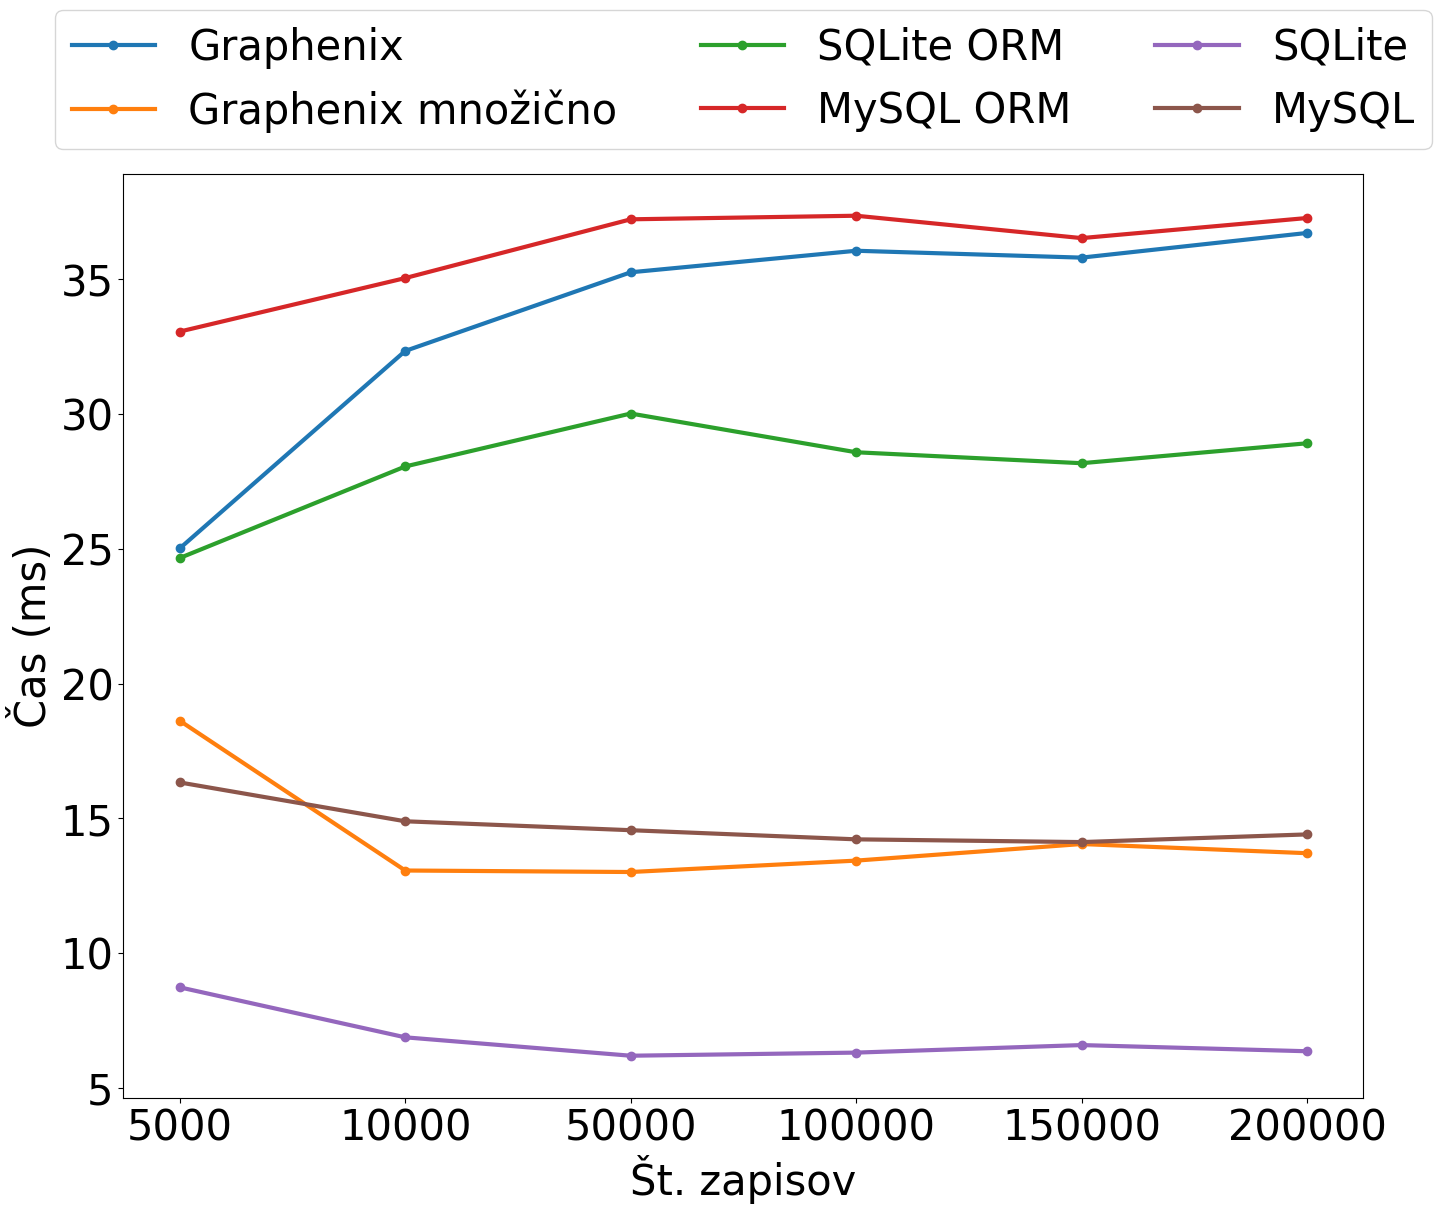
\includegraphics[width=0.70\textwidth, angle=0]{singleinsert.png}}
        \caption{Normaliziran čas vnašanja podatkov}
        \label{vnos}
    \end{figure}

    \noindent
    Prva ugotovitev, ki jo lahko izpeljemo iz grafa, je, da je vstavljanje podatkov z uporabo ORM precej počasnejše v primerjavi z neposrednim vstavljanjem preko SQL ukazov. Uporaba ORM zahteva ustvarjanje instanc objektov, kar vodi v dodatne časovne zakasnitve.

    Na splošno lahko opazimo, da je SQLite prevladujoč pri hitrosti vstavljanja. Razlog, da MySQL ni tako hiter, je dokaj enostaven. MySQL DBMS teče na strežniku in vso komunikacijo opravlja prek vgrajenega protokola, kjer se podatki prenašajo z uporabo TCP/IP paketov, kar ni tako učinkovito, kot uporaba I/O operaciji v SQLite.

    V primeru Graphenix DBMS vstavljanje ni izvedeno v klasični množični obliki, saj je vsatvljanje vsakega zapisa ločen dostop do datoteke. V analizi sta predstavljena dva pristopa vnašanja z uporabo razvite knjižnice. V primeru množičnega vnašanja gre za direkten klic funkcije jedra za vnašanje podatkov in ne potrebujemo kreirati instanc objektov, kar je bilo tudi glavno ozko grlo pri vnašanju podatkov z uporabo ORM.

    Pomemben dejavnik pri vnašanju podatkov je tudi dodatna varnost, ki jo zagotavljata SQLite in zlasti MySQL. Oba sistema imata dnevnike, ki v primeru napake omogočata povrnitev celotne baze podatkov v stanje pred vnašanjem. Posledično v primeru napake ali prekinitve v Graphenix DBMS tvegamo imeti neveljavne zapise v bazi podatkov.

    \subsection{Vnašanje z dodatnim indeksiranim poljem}

    V drugem scenariju, gre za enakovredno vnašanje prvemu, vendar z dodatkom definicije indeksa na atributu entitete (indeks je definiran na celoštevilskem polju, kjer je vsaka vrednost unikatna).
    
    \begin{figure}[H]
        \centerline{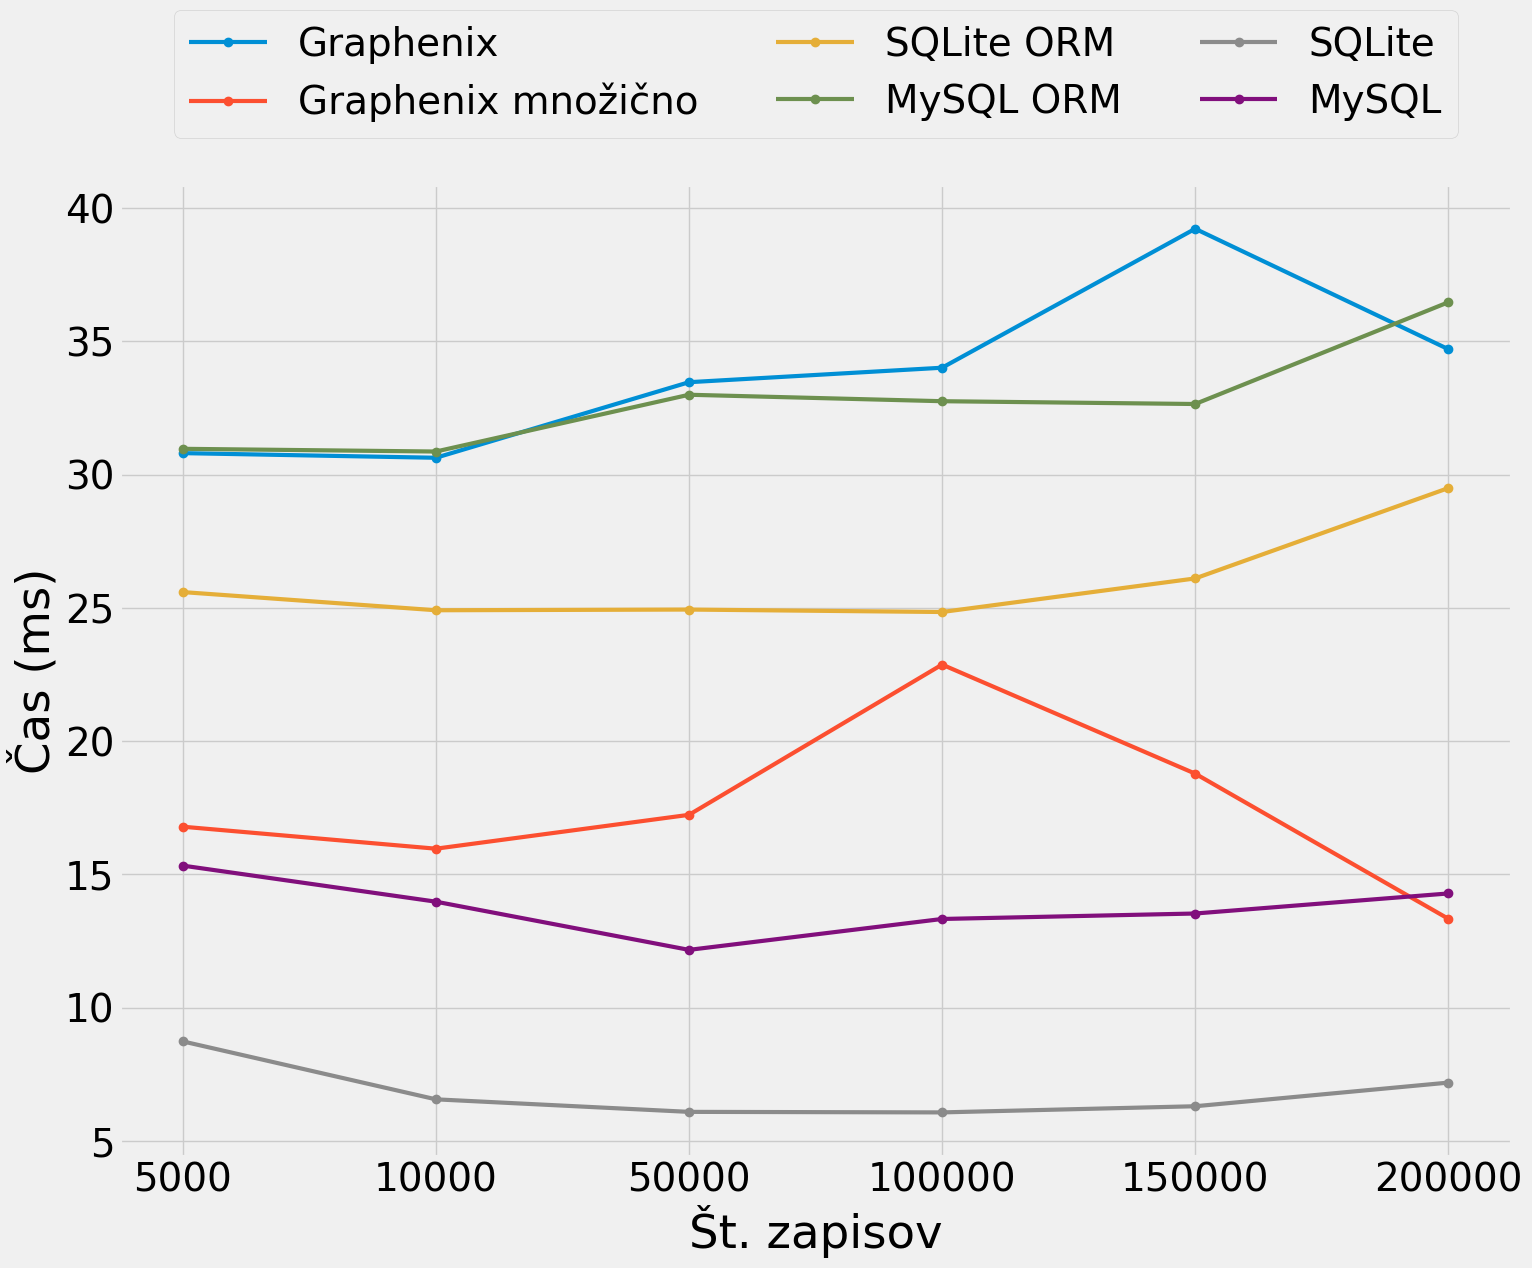
\includegraphics[width=0.70\textwidth, angle=0]{indexinsert.png}}
        \caption{Normaliziran čas vnašanja podatkov z dodatnim vnašanjem v B+ strukturo}
        \label{index_vnos}
    \end{figure}

    \noindent
    Iz grafa lahko razberemo, da iz vidika hitrosti vstavljanja še vedno prevladuje SQLite. Za razliko od predhodnega scenarija \ref{vnos}, pa tokrat MySQL v večini primerov postane bolj učinkovit kot Graphenix.

    V vseh treh DBMS je indeksiranje realizirano z uporabo B drevesa. Kljub temu, pa je razlika v načinu vnašanja podatkov, namreč naša implementacija B drevesa ne izkorišča algoritma za množično vstavljanje v drevo. MySQL in SQLite za vstavljanje uporabljata algoritem množičnega vstavljanja in posledično čas vstavljanja v drevo nima bistvenega vpliva na celoten čas vstavljanja.
 
    \section{Velikosti podatkovnih baz na disku}
    \label{size_analysis}

    Glede na prva dva scenarija smo pripravili tudi stolpčni grafikon \ref{velikosti}, kjer primerjamo porabo prostora na disku posameznega DBMS (gre za baze podatkov z milijon zapisi). 
    
    \begin{figure}[H]
        \centerline{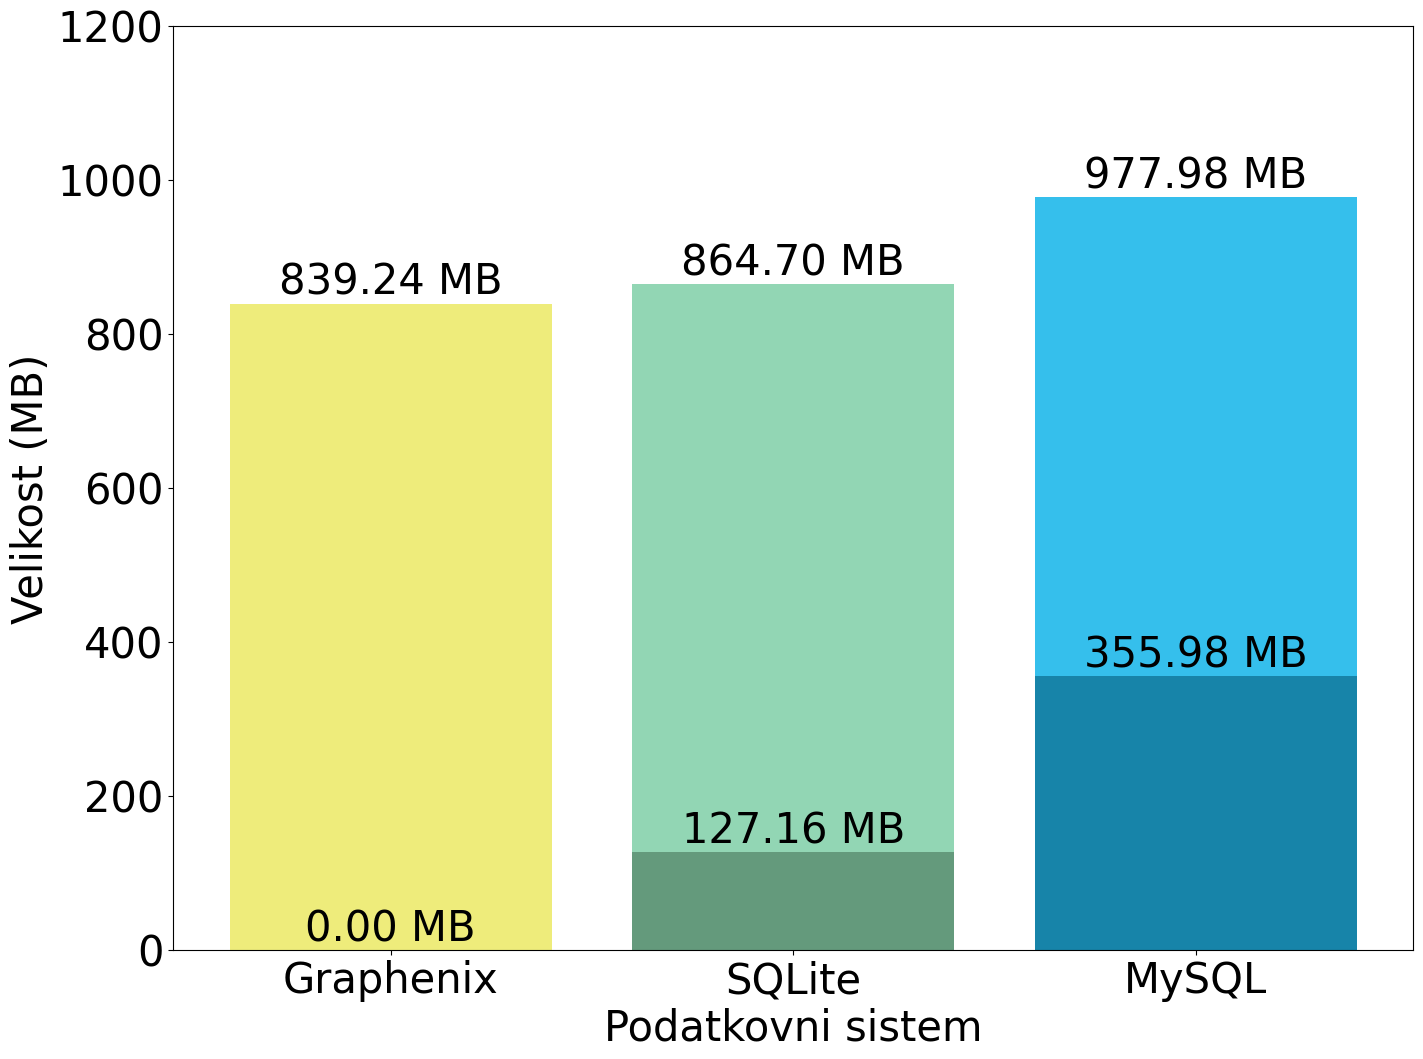
\includegraphics[width=0.7\textwidth, angle=0]{sizes.png}}
        \caption{Prostorska poraba na nivoju diska posameznega DBMS}
        \label{velikosti}
    \end{figure}

    \noindent
    Iz grafa takoj opazimo, da je Graphenix DBMS najbolj potraten iz vidika porabe prostora. Razlog se skriva v načinu shranjevanja tekstovnih vrednosti. SQLite in MySQL uporabljata podatkovne strukture, ki ob shranjevanju prinesejo še dodatno optimizacijo porabe prostora, saj uporabita le toliko prostora kot je potrebno. V primeru Graphenix, pa je dolžina tekstovnih polji točno določena in v primeru, da polje definiramo kot ``Field.String(size=50)`` pomeni, da bo vsak zapis ne glede na dolžino zavzel 50 bajtov.

    V temnem delu stolpca je prikazana razlika velikosti z in brez uporabe indeksne strukture. DBMS z najnižjo porabo prostora iz vidika velikosti indeksne strukture je SQLite. Razlog za nižjo porabo se nahaja v velikosti posameznega vozlišča in samem algoritmu vstavljanja v drevo, ki vpliva tudi na delitev vozlišč tekom vnašanja.

    \section{Primerjava poizvedb na eni entiteti}

    Za tretji scenarij je pripravljena analiza, kjer izmerimo čas izvajanja na preprosti poizvedbi branja brez kakršnih koli omejitev.
    
\begin{minted}[breaklines]{SQL}
SELECT * FROM users
\end{minted}
    

    \begin{figure}[H]
        \centerline{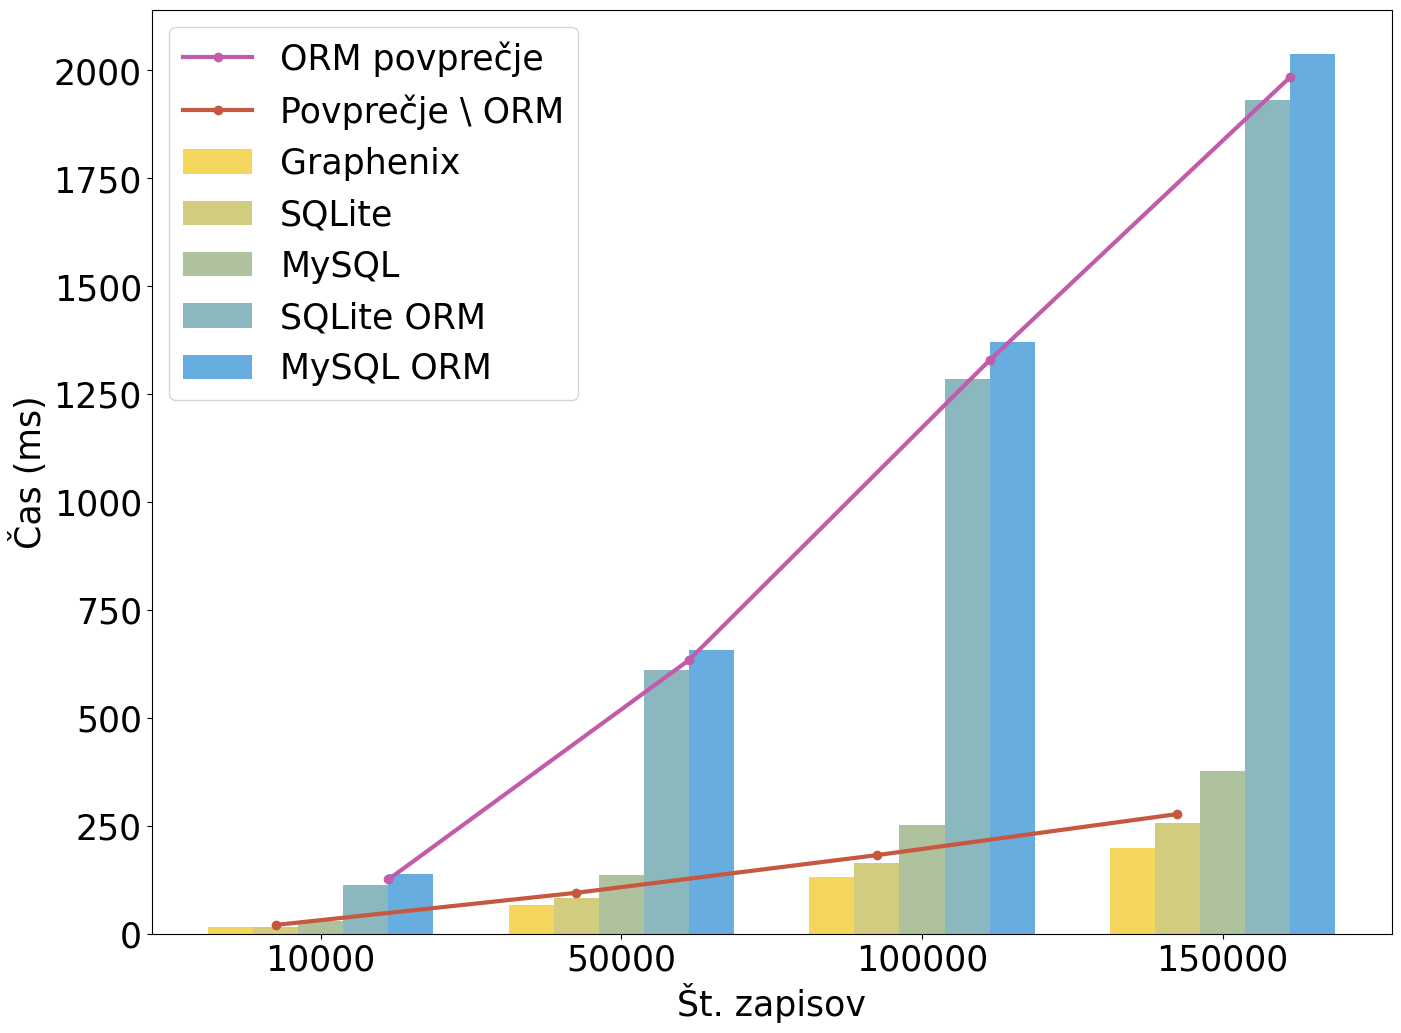
\includegraphics[width=0.7\textwidth, angle=0]{singleread.png}}
        \caption{Branje brez dodatnih parametrov znotraj poizvedbe}
        \label{branje}
    \end{figure}

    \noindent
    Iz grafa je jasno razvidno, da uporaba ORM ni dobro pripravljena za masovno nalaganje podatkov, saj se ponovno kreirajo instance, kar predstavljaj več kot 70\% delež celotnega branja. V primeru MySQL se ponovno pojavi tudi nekaj dodatne zakasnitve zaradi načina prenosa podatkov preko TCP/IP protokola.

    \subsection{Branje s filtriranjem, urejanjem in omejevanjem podatkov}

    V drugem scenariju branja podatkov iz ene entitete dodamo še omejitev na tip uporabnikov (želimo le administratorje). Poleg tega, pa je dodano tudi urejanje podatkov in dodana omejitev števila zapisov (želimo prvih 500 zapisov urejenih po točkah uporabnika).

\begin{minted}[breaklines]{SQL}
SELECT * FROM users
WHERE is_admin = 1
ORDER BY points, id
LIMIT 500
\end{minted}
    
    \begin{figure}[H]
        \centerline{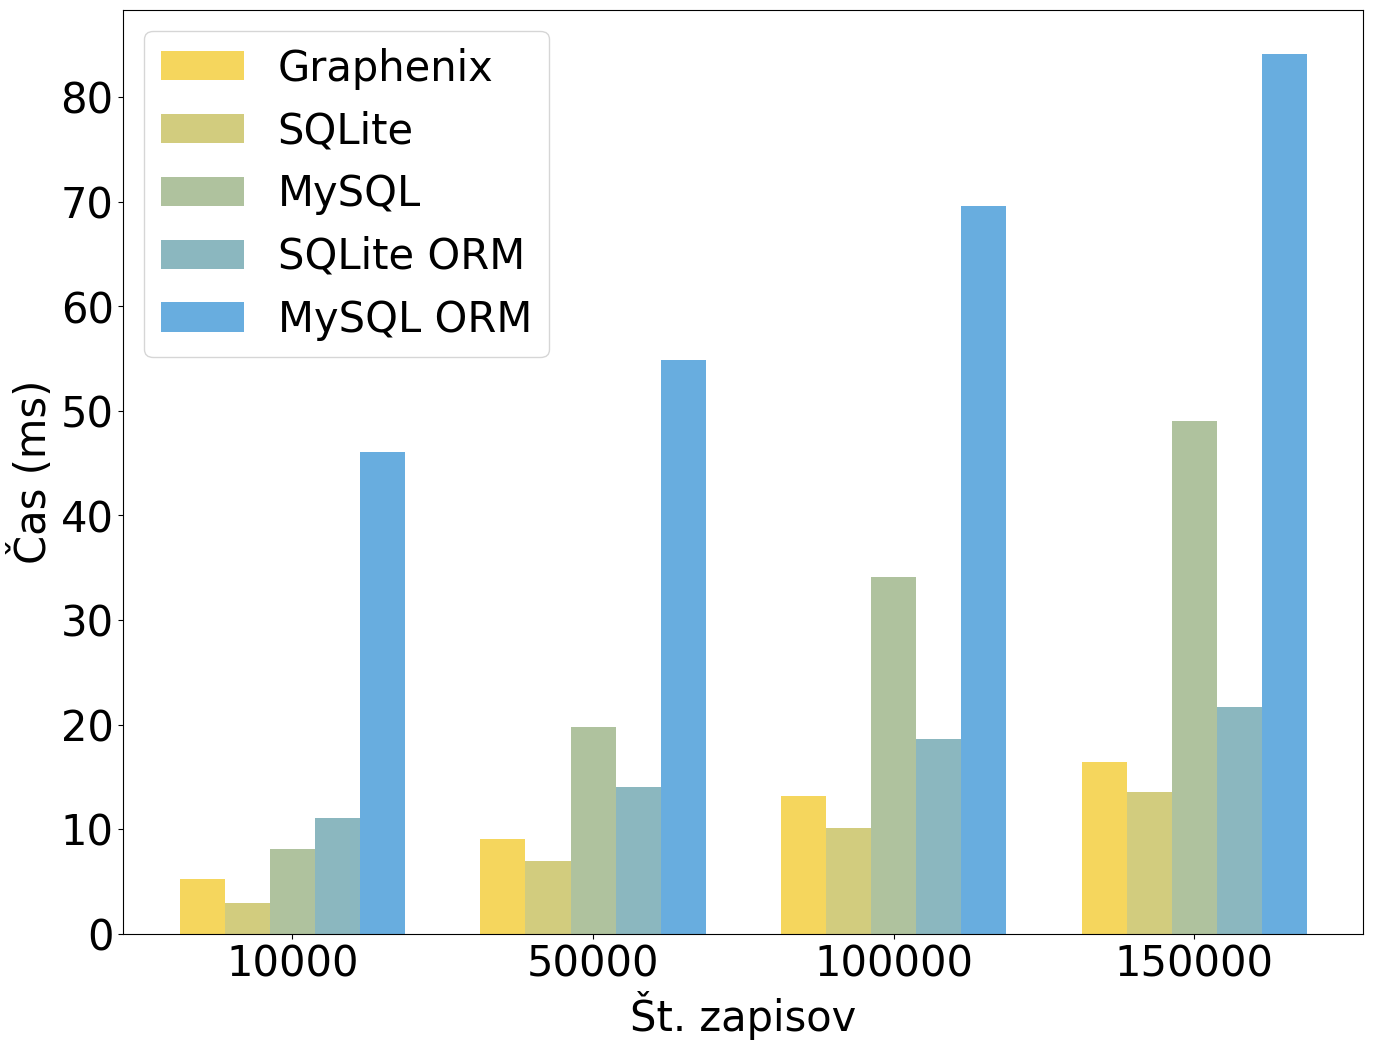
\includegraphics[width=0.7\textwidth, angle=0]{queryread.png}}
        \caption{Branje z dodanim filtriranjem in urejanjem zapisov}
        \label{queryread}
    \end{figure}

    \noindent
    Sam čas izvajanja posameznega branja je relativno nizek, v vseh primerih je bilo branje izvedeno v manj kot 100 ms. Opazimo, da zakasnitve kreiranja instanc pri ORM tukaj ne pridejo toliko do izraza, saj je potrebno kreirati le 500 instanc. Do večjega izraza pridejo zakasnitve, ki jo za prenos podatkov prinaša TCP/IP protokol, kar je videno v primerih uporabe MySQL.

    \section{Primerjava poizvedb z uporabo relaciji}
    \label{join_lbl}

    V scenariju definiramo poizvedbo, kjer izvedemo nabor podatkov iz dveh entitet. Št. zapisov je določeno s številom uporabnikov. Za vsakega uporabnika, pa je bilo vnesenih še 10 nalog, ki so vezane preko tujega ključa ``user\_id`` v entiteti nalog.
    
\begin{minted}[breaklines]{SQL}
SELECT * FROM users 
INNER JOIN tasks ON tasks.user_id = users.id
\end{minted}

    \begin{figure}[H]
        \centerline{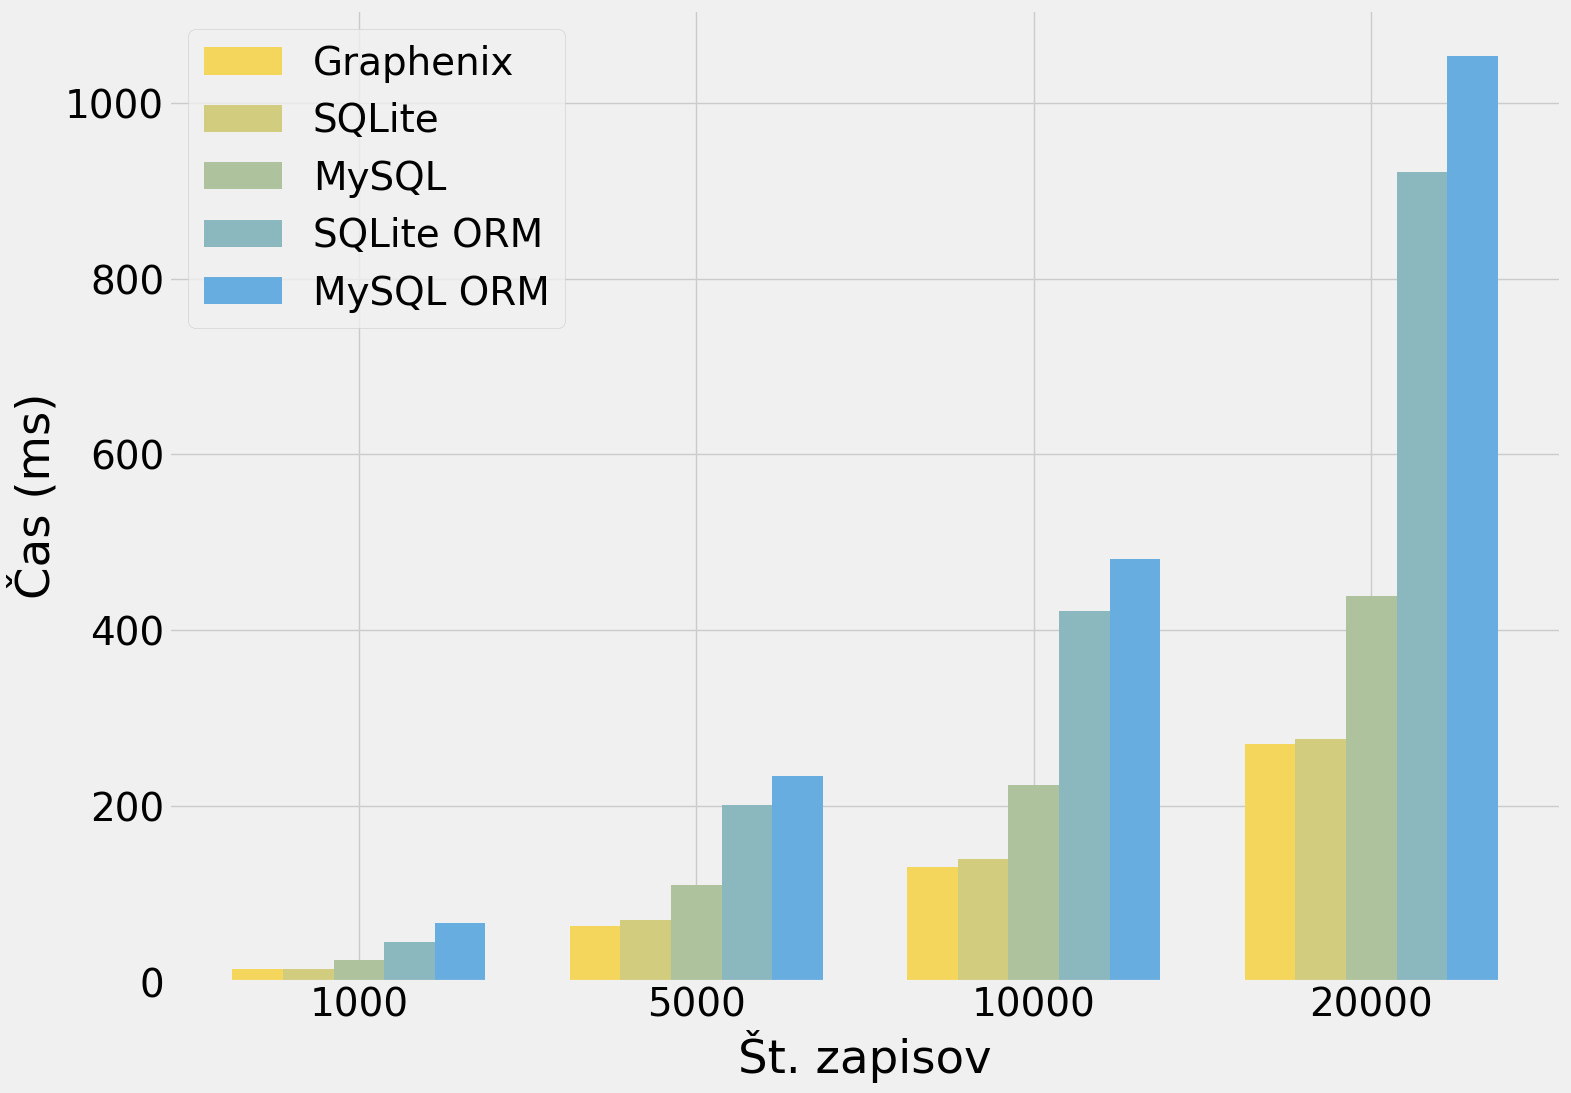
\includegraphics[width=0.6\textwidth, angle=0]{join.png}}
        \caption{Poizvedovanje podatkov iz dveh entitet hkrati – uporabniki in njihove naloge}
        \label{join}
    \end{figure}

    \noindent
    Ponovno se izkaže, da ORM s seboj prinese dodatne zakasnitve zaradi kreiranja instanc. Za razliko od prejšnjih scenarijev pride tukaj do razlike v sami strukturi rezultata.
    
    \begin{itemize}
        \item ORM – podatki so v gnezdeni obliki, kjer imamo za vsakega izmed uporabnikov seznam njegovih nalog.
        \item Brez – podatki so v obliki kartezičnega produkta oz. matrike in imamo za vsakega uporabnika toliko zapisov, kot ima uporabnik sporočil.
    \end{itemize}

    \noindent
    Graphenix deluje po principu ORM in imamo gnezdeno strukturo podatkov. Kljub temu, pa zaradi združevanja na nivoju programskega jezika C++ poizvedba steče v primerljivem času poizvedbam, ki ne uporabljajo ORM.
    
    \section{Izvedba agregacijske poizvedbe}

    V scenariju izvedbe agregacije uporabljamo strukturo, ki smo jo pripravili v prejšnjem scenariju \ref{join_lbl}.

    V poizvedbi naloge združujemo po uporabnikih in za vsakega uporabnika pridobimo število nalog, ki mora biti v vseh primerih 10. Poleg tega, pa glede na atribut ``created\_at`` pridobimo tudi datum zadnje naloge uporabnika.
    
\begin{minted}[breaklines]{SQL}
SELECT user_id, COUNT(*) AS 'count', 
       MAX(created_at) AS 'latest' 
FROM tasks GROUP BY user_id
\end{minted}

    \begin{figure}[H]
        \centerline{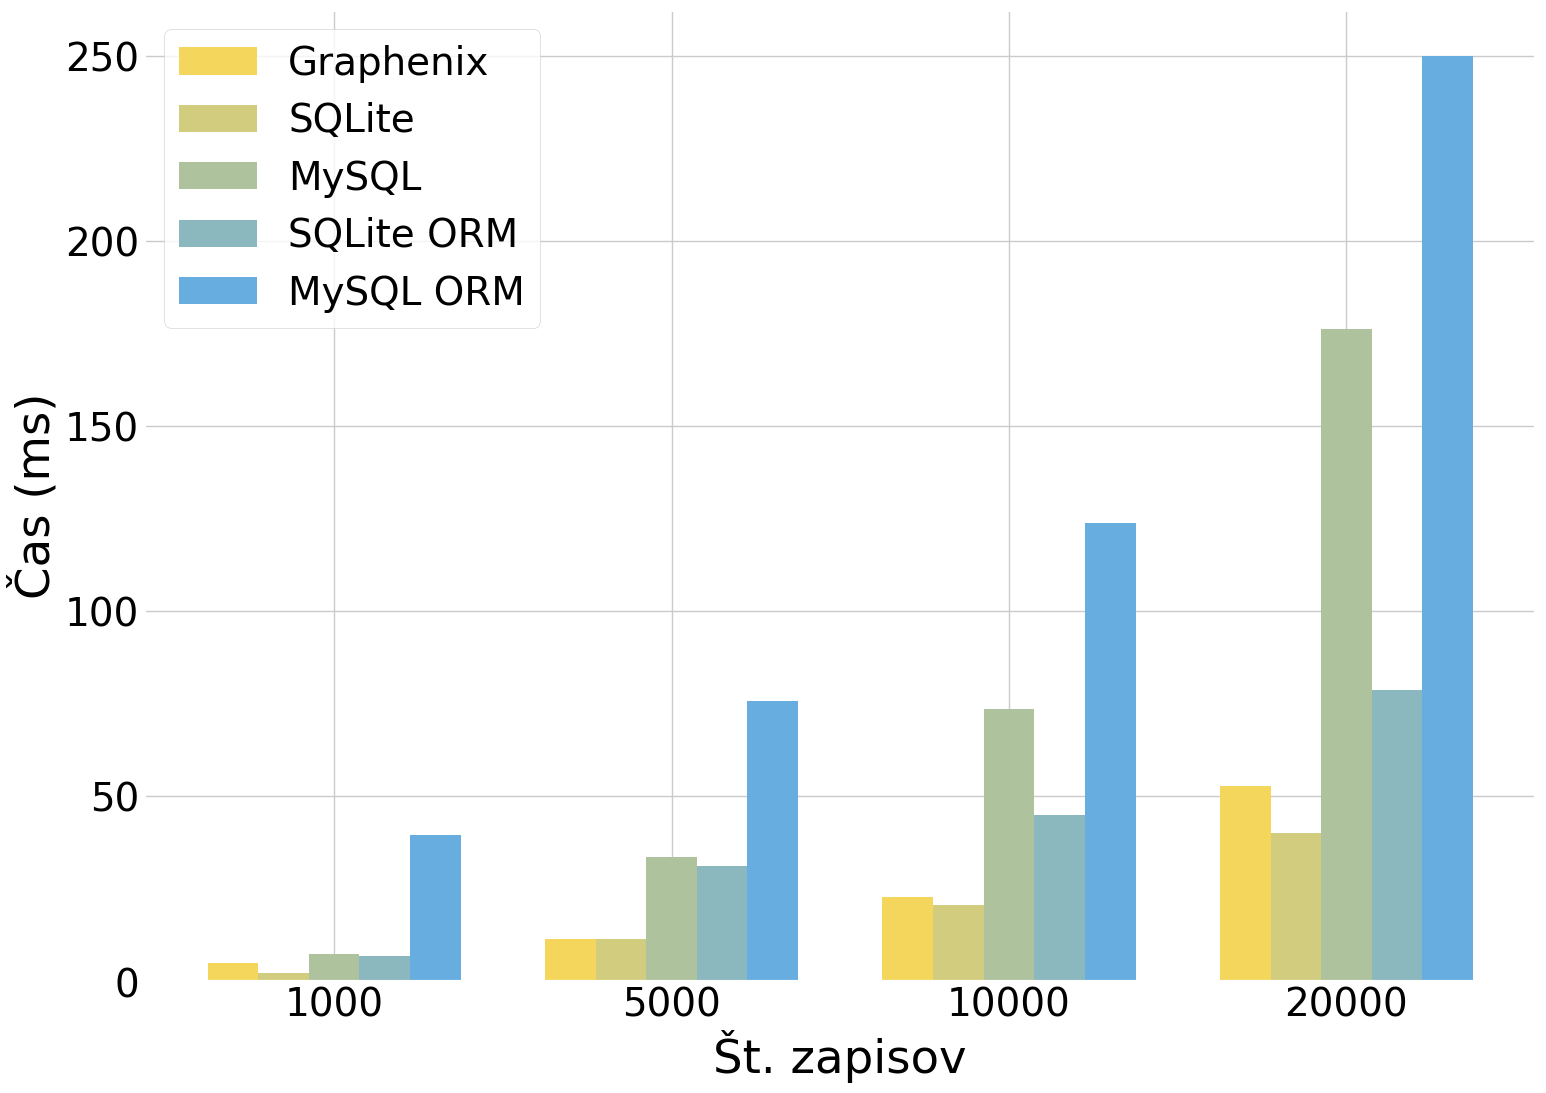
\includegraphics[width=0.6\textwidth, angle=0]{agg.png}}
        \caption{Uporaba agregacijskih metod}
        \label{agg}
    \end{figure}

    \noindent
    V tem scenariju rezultat poizvedbe ni predstavljen, kot instance objektov, saj vedno kreiramo prilagojen tip rezultata, ki vsebuje identifikator uporabnika, število nalog in zadnji datum naloge za vezanega uporabnika.

    Rezultati sicer dobro sledijo trendom iz predhodnih scenarijev – MySQL zaradi načina prenosa podatkov potrebuje nekoliko več časa, poleg tega pa se ponovno pozna razlika uporabe ORM in uporaba SQL poizvedb. Graphenix pa je ponovno primerljiv uporabi SQLite brez ORM.

    \section{Pohitritve s pomočjo indeksiranja}

    Kot zadnji scenarij je predstavljen eden izmed najbolj kritičnih segmentov DBMS – pohitritev iskanja s pomočjo indeksiranja podatkov. V scenariju primerjamo pristop brez in z uporabo indeksiranja.
    
\begin{minted}[breaklines]{SQL}
SELECT * FROM users
WHERE points = 5432
\end{minted}

    \noindent
    Na grafu \ref{old_speedup} je prikazano iskanje zapisa nad entiteto z \num{100000} zapisi.

    \begin{figure}[H]
        \centerline{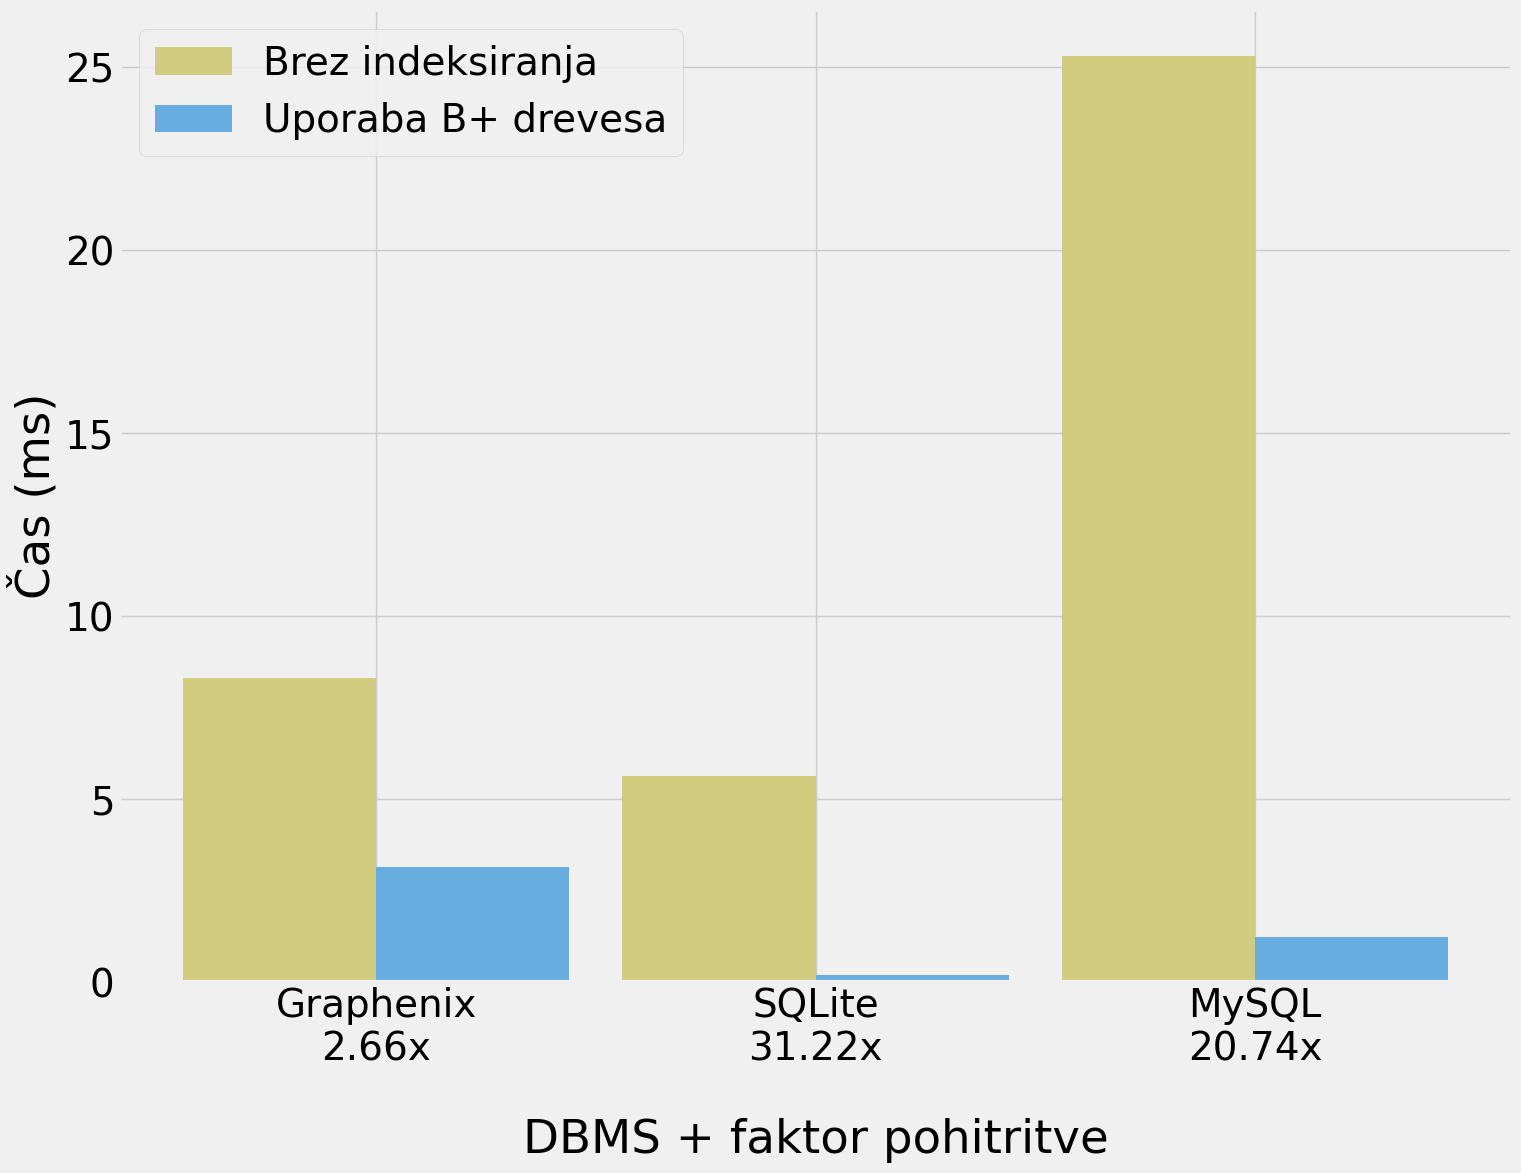
\includegraphics[width=0.7\textwidth, angle=0]{indexing_speedup_100000.png}}
        \caption{Iskanje specifičnega zapisa ($N = \num{100000}$)}
        \label{old_speedup}
    \end{figure}

    \noindent
    Iz grafa hitro razberemo, da je pohitritev v Graphenix DBMS drastično manjša, kot je to v primeru SQLite in MySQL.

    \subsection{Optimizacija v metodi filtriranja zapisov}

    Zaradi bistveno slabšega rezultata pri iskanju smo se lotili profiliranja posameznih segmentov programske kode za nabor podatkov.

    Kaj hitro smo prišli do ugotovitve, da težava ni bil proces iskanja v B drevesu, temveč je bila težava branje zaglavja entitete. Metoda za branje podatkov iz posamezne entitete je delovala, tako da je najprej prebrala celotno datoteko zaglavja entitete in za posamezen identifikator zapisa pridobila še odmik v matriki zapisov. Izkazalo se je, da je ta proces v zgornjem scenariju predstavljal nekje $\approx 85$\% izvajalnega časa.

    V namen hitrejšega izvajanja se branja celotnega zaglavja v primeru, da imamo že vnaprej določene identifikatorje, ki jih iščemo in je teh manj kot $IX\_THRESHOLD$ izognemo. Konstanta predstavlja mejo za branje celotnega zaglavja in je v trenutni implementaciji nastavljena na \num{100}.
    
    \begin{figure}[H]
        \centerline{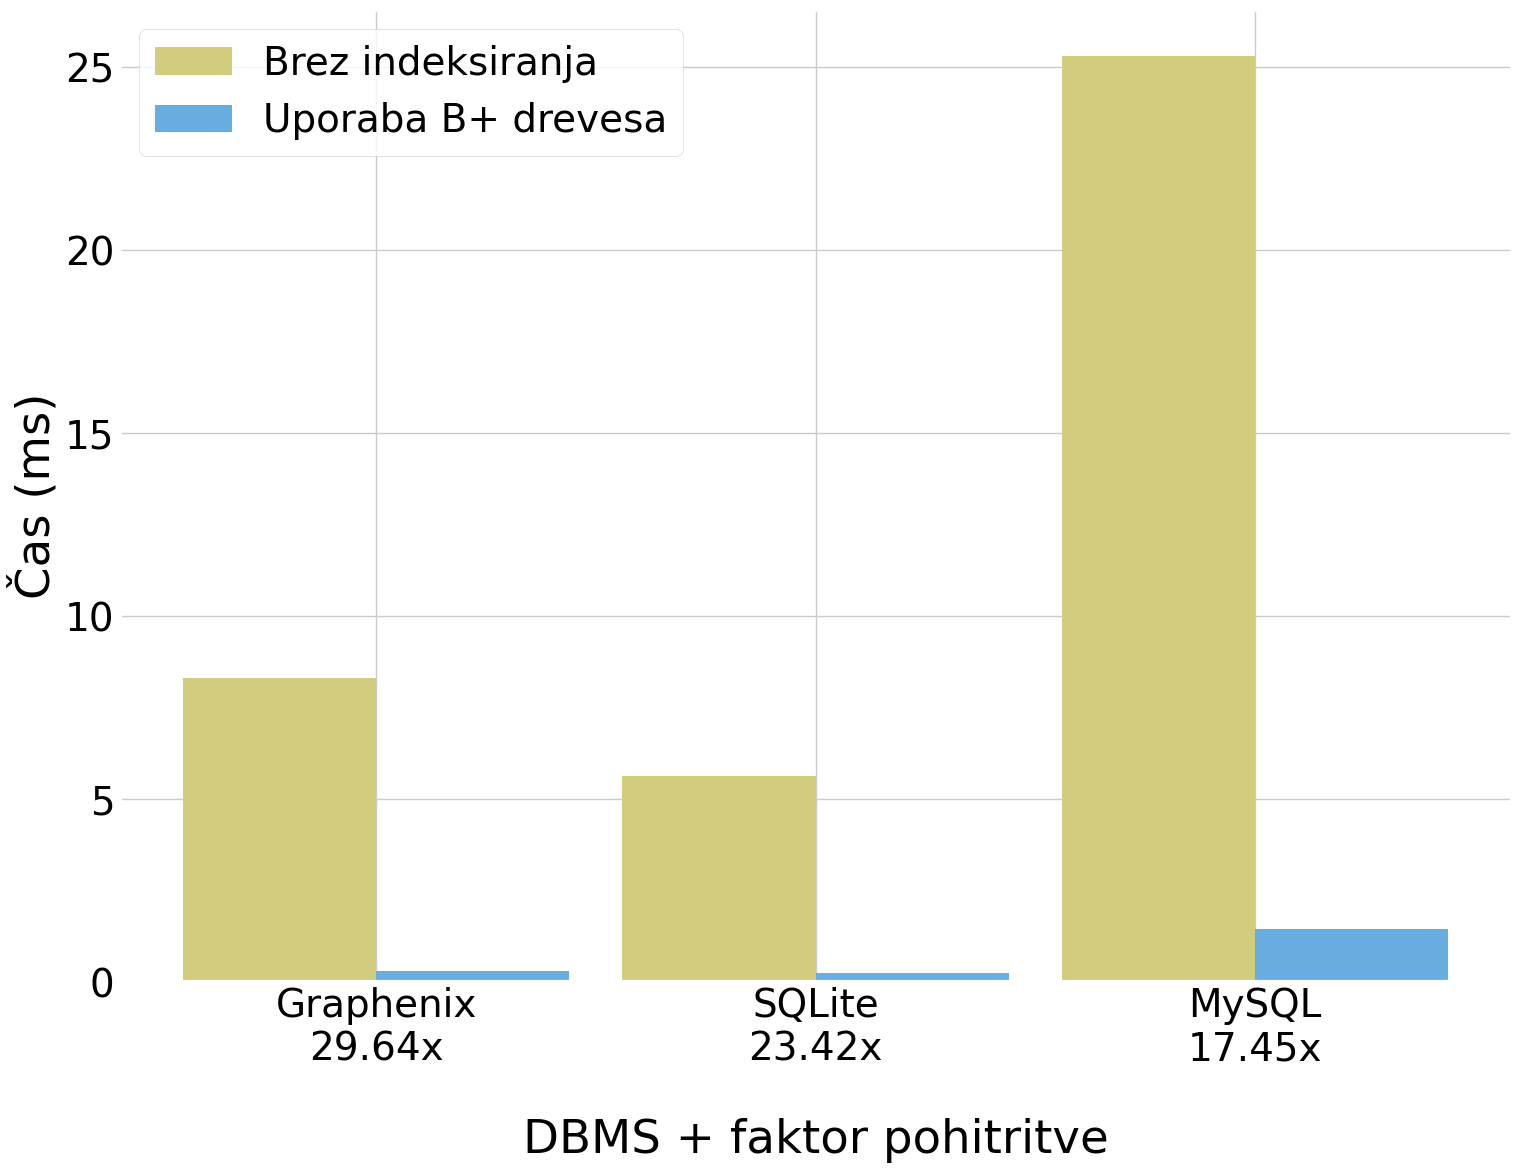
\includegraphics[width=0.75\textwidth, angle=0]{indexing_speedup_100000_v2.png}}
        \caption{Iskanje specifičnega zapisa ($N = \num{1000000}$ z optimizacijo)}
        \label{idx_speedup}
    \end{figure}

    \noindent
    Po implementirani optimizaciji opazimo bistveno izboljšavo, kar se tiče časa iskanja. Sedaj se čas in faktor pohitritve lahko primerjata z MySQL in SQLite.

    \subsubsection{Analiza iskanja nad večjo bazo podatkov}

    Na grafu \ref{idx_speedup_2} je prikazana še pohitritev enake poizvedbe, kot v zgornjem scenariju. V tem primeru, pa je število vseh uporabnikov \num{1000000}.
    
    \begin{figure}[H]
        \centerline{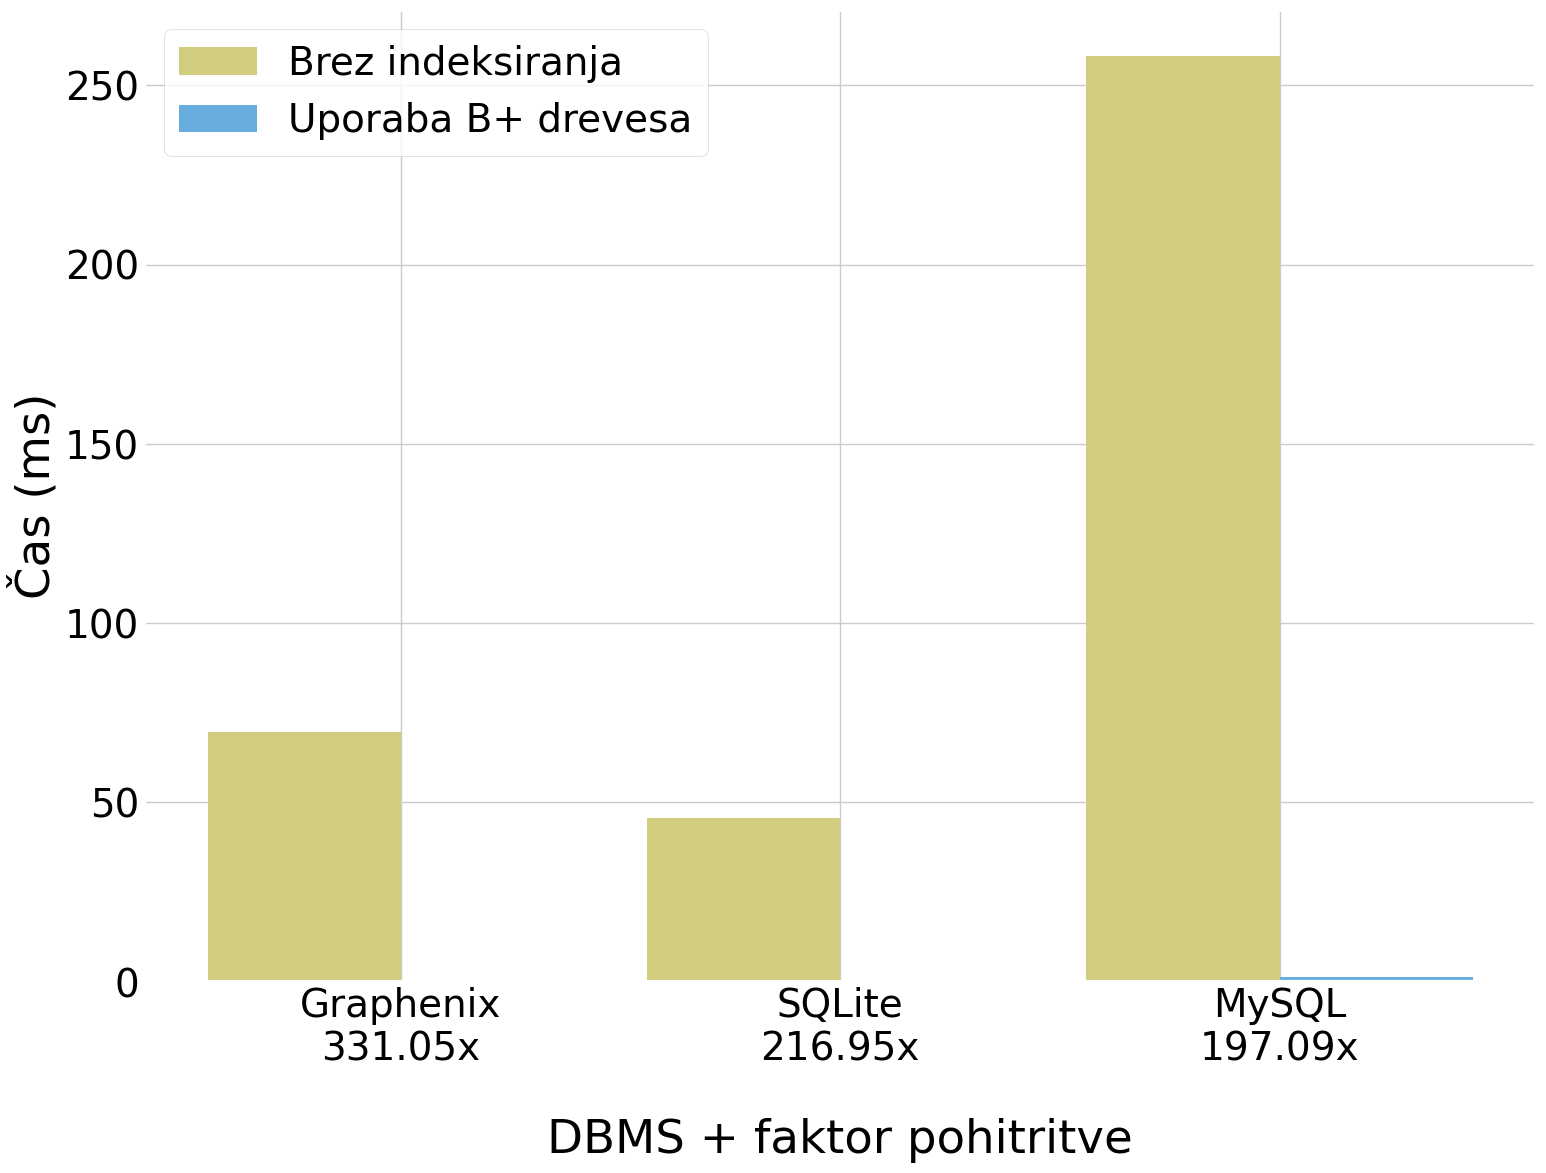
\includegraphics[width=0.75\textwidth, angle=0]{indexing_speedup_1000000_v2.png}}
        \caption{Iskanje specifičnega zapisa ($N = \num{1000000}$ z optimizacijo)}
        \label{idx_speedup_2}
    \end{figure}

    \noindent
    Iz grafa razberemo, da v vseh treh izvedbah zapis najdemo v manj kot 2 ms, kar tudi v vseh treh scenariji predstavlja več 100x pohitritev. Nekaj zakasnitve se sicer vseeno pojavi iz strani MySQL, kar je glede na predhodne scenarije pričakovano.

    \subsubsection{Idealni pogoji za indeksiranje}
    Pomembno je omeniti, da je scenarij zelo prilagojen uporabi indeksiranja, saj v scenariju iskanja, kjer vrednosti niso unikatne učinkovitost indeksa zelo hitro pade. Poleg tega je bilo iskanje izvedeno, kot iskanje specifične vrednosti v drevesu, medtem, ko če bi iskali širši interval vrednosti bi se ponovno oddaljili od časovne zahtevnosti $O(log_M(N))$ in približali $O(N)$.

    Če potegnemo rdečo nit je jasno, da se pri odločanju o uporabi indeksov odpira kompleksno vprašanje, ki zahteva premišljeno obravnavo. Odgovornost za to odločitev se prepušča razvijalcem, pri čemer je ključnega pomena, da se kot razvijalci zavedamo optimizaciji in pasti, ki izvirajo iz uporabe B dreves za indeksiranje. Poleg tega je nujno, da poznamo naravo podatkov in zahtev aplikacije, saj je optimizacija z indeksiranjem smiselna le v določenih kontekstih.

\chapter{Scenariji oz. primeri uporabe}
\label{ch3}

    V tem poglavju sta predstavljena dva primera uporabe knjižnice Graphenix. V prvem primeru se knjižnica uporablja kot dodatek strežniški aplikaciji v namen beleženja podatkov. V drugem scenariju, pa je predstavljen razvoj preproste namizne aplikacije, kjer knjižnico uporabljamo za trajno shranjevanje podatkov. Oba primera skušata na praktičen način predstaviti dobre strani uporabe Graphenix knjižnice.

    \section{Strežniško beleženje podatkov}

    Pogosta uporaba programskega jezika Python je na strani strežniških aplikaciji. Na tem področju je beleženje sprememb in zahtev kritično. Z uporabo pripravljene knjižnice je prilagojeno beleženje podatkov lahko zelo preprosto.

    \subsection{Aplikacija, ki služi kot osnova za modul beleženja}

    V prvi fazi si lahko za primer pripravimo preprosto strežniško aplikacijo, ki uporablja Flask \cite{FLASK_GITHUB} ogrodje. Znotraj aplikacije smo definirali vsega eno vhodno točko, in sicer ``get-range``, kjer lahko poljubno nastavljamo tri HTTP GET parametre, to so ``start``, ``end`` in ``step``, kjer ima vsak od teh parametrov tudi privzete vrednosti.
    
\begin{minted}{python}
app = Flask(__name__)
@app.route('/get-range')
def get_range(request):
    start = int(request.args.get('start', 0))
    end = int(request.args.get('end', 10))
    step = int(request.args.get('step', 1))
    return jsonify({'Range': list(range(start, end, step))})
app.run()
\end{minted}

    \subsection{Kreiranje sheme za beleženje podatkov}
\begin{minted}{python}
class ReqInfo(gx.Model):
    route = gx.Field.String(size=255)
    timestamp = gx.Field.DateTime().as_index()
    route_req = gx.Field.String(size=1024)
    route_res = gx.Field.String(size=1024)
    resp_code = gx.Field.Int()

logging = gx.Schema('logging', models=[ReqInfo])
if not logging.exists():
    logging.create()
\end{minted}

    \noindent
    V zgornjem kosu programske kode pripravimo razred, ki predstavlja entiteto, ki skupaj z definiranimi atributi predstavlja strukturo podatkov, katere bomo tekom delovanja naše aplikacije beležili. V drugi fazi, pa moramo kreirati še shemo, v kateri definiramo naziv in vse razrede oz. entitete, ki bodo del naše baze podatkov.

    \subsection{Dekorator za dinamično dodajanje beleženja}

    V namen beleženja znotraj vhodnih točk strežniške aplikacije bomo uporabili lasten dekorator.
    Dekorator je vzorec,  ki omogoča dinamično dodajanje funkcionalnost obstoječi funkciji, ne da bi spreminjali njeno strukturo. Tekom izvedbe notranje funkcije lahko argumente in različne segmente izvajanja prestrežemo in jih prilagodimo glede na naše zahteve.
    
\begin{minted}[breaklines]{python}
def route_with_log(route):
    def decorator(f):
        @wraps(f)
        def wrapper(*args, **kwargs):
            try:
                response = f(request, *args, **kwargs)
            except Exception as err:
                response = None

            ReqInfo(
                route=route,
                timestamp=datetime.now(),
                route_req=json.dumps(dict(request.args)),
                route_res=response.get_data(as_text=True) if response else '',
                resp_code=response.status_code if response else 500
            ).make()

            return response
        
        app.add_url_rule(route, view_func=wrapper)
        return wrapper
    return decorator
\end{minted}

    \noindent
    V primeru našega dekoratorja $route\_with\_log(...)$ vhodni točki dodamo še funkcionalnost beleženja podatkov.

    \subsection{Branje zapisanih podatkov}

    V končni fazi je glavna prednost uporabe pripravljene knjižnice dobra struktura shranjenih podatkov, ki omogoča preprosto obdelavo in manipulacijo. Posledično nam je omogočeno tudi bistveno več načinov pridobivanja statističnih podatkov, saj lahko le-te poljubno filtriramo, grupiramo, združujemo in razvrščamo. Na nivoju administratorske aplikacije lahko nato prožimo različne poizvedbe nad našo bazo podatkov.

    \subsubsection{Izpis zadnjih treh zahtevkov}

\begin{minted}{python}
_, reqs = ReqInfo.order(ReqInfo.timestamp.desc()).limit(3).all()
... 
ReqInfo(id=3, route=/get-range, timestamp=2023-07-16 03:02:15, 
    route_req={}, route_res={"Range":[0,1,2,3,4,5,6,7,8,9]},
    resp_code=200)
    
ReqInfo(id=2, route=/get-range, timestamp=2023-07-16 03:02:13, 
    route_req={"start": "3"}, route_res={"Range":[3,4,5,6,7,8,9]},
    resp_code=200)
    
ReqInfo(id=1, route=/get-range, timestamp=2023-07-16 03:02:05,
    route_req={"start": "15", "end": "10", "step": "-3"},
    route_res={"Range":[15,12]}, resp_code=200)
\end{minted}

    \newpage
    \subsubsection{Statističen pregled zahtevkov}

    Podatke lahko v pripravljenem DBMS tudi grupiramo, in sicer z uporabo $.agg(...)$ metode v poizvedbi. Znotraj metode definiramo polje po katerem grupiramo podatke, kot tudi agregacije, ki jih želimo izvesti.
    
\begin{minted}{python}
route_stats = ReqInfo\
    .agg(by=ReqInfo.route, count=gx.AGG.count())
\end{minted}

    \noindent
    Z zgornjo poizvedbo dobimo število zahtevkov grupirano po vhodni točki aplikacije. 

    \subsubsection{Izpis napak v zadnjem dnevu}

    Za nabor napak v zadnjem dnevu, lahko preprosto izvedemo poizvedbo, kjer zahtevamo, da je status odgovora $>= 400$, kar pri HTTP zahtevkih predstavlja razpon napak. Poleg tega, pa dodamo še zahtevo, da mora biti datum napake večji, kot včerajšnji datum ob enaki uri. Za konec zapise uredimo po datumu napake.
    
\begin{minted}{python}
count, api_errors = ReqInfo\
    .filter(
        ReqInfo.resp_code >= 400,
        ReqInfo.timestamp > datetime.now() - timedelta(days=1)
    )\
    .order(ReqInfo.timestamp.desc())\
    .all()
\end{minted}

    \subsubsection{Izvoz vseh podatkov v .csv datoteko}

    DBMS omogoča tudi izvoz v {\tt.csv} datoteko, ki za nekatere uporabnike lahko pomeni lažjo obdelavo podatkov, poleg tega, pa lahko predstavlja tudi varnostno kopijo podatkovne baze v ločeni datoteki.

    Za izvoz potrebujemo najprej izvesti nabor vseh podatkov, nato pa s pomočjo privzetega pretvornika podatke izvozimo v datoteko s pomočjo metode ``dump2csv``, ki prejme dva parametra – podatke in naziv izvozne datoteke.
    
\begin{minted}{python}
_, all_reqs = ReqInfo.all()
gx.ViewSearilizer.default().dump2csv(all_reqs, 'export.csv')
\end{minted}

    \section{Namizna aplikacija za upravljanje stroškov}

    V tem sklopu je predstavljen razvoje preproste namizne aplikacije za upravljanje stroškov. Aplikacija omogoča pregled stroškov, vnašanje, urejanje in brisanje, ter statističen pregled, kjer so stroški grupirani glede na kategorije.

    \subsection{Zaslonski pregled aplikacije}
    Na sliki \ref{home_screen} je prikazan začetni zaslon, kjer imamo v obliki seznama pregled vseh stroškov uporabnika in ob tem še zaslon za urejanje ali kreiranje novega stroška. 
    
    \begin{figure}[H]
        \centerline{\includegraphics[width=1\textwidth, angle=0]{app_psd.png}}
        \caption{Seznam stroškov z možnostjo vnašanja in urejanja}
        \label{home_screen}
    \end{figure}

    \noindent
    Za vsak posamezen strošek na skupnem prikazu sta definirani akciji brisanja in urejanja. Poleg tega lahko stroške glede na naziv, ceno in kategorijo tudi urejamo. Omogočeno je tudi filtriranje stroškov po nazivu in prikazovanje po straneh.

    Na desnem zaslonu je predstavljen obrazec, do katerega dostopamo preko urejanja ali kreiranja novega stroška. Gre za preprost obrazec, kjer določimo naziv, ceno in kategorijo posameznega stroška.

    \subsubsection{Statističen pregled stroškov}
    Na sliki \ref{stats_screen} je prikazan statističen pregled stroškov, kjer so ti grupirani glede na kategorijo. Gre za tabelarni prikaz, kjer imamo za vsako kategorijo naziv, datum zadnjega stroška, število stroškov in vsoto cen vseh stroškov posamezne kategorije.

    \begin{figure}[H]
        \centerline{\includegraphics[width=1\textwidth, angle=0]{stats_psd.png}}
        \caption{Statističen pregled stroškov}
        \label{stats_screen}
    \end{figure}

    \subsection{Aplikacija iz vidika kode}

    Grahepnix je dobra izbira, saj gre za relativno nezahtevno aplikacijo, kjer ne potrebujemo skrbeti za več hkratnih dostopov do baze podatkov, poleg tega pripravljen ORM omogoča zelo preprost pristop za manipulacijo podatkov.

    Za izris uporabniškega vmesnika aplikacija uporablja BeeWare \cite{BEE_WARE}, ki omogoča medplatformski razvoj programske opreme, kar pomeni, da lahko isto kodo uporabimo za več različnih operacijskih sistemov.

    \subsubsection{Stuktura podatkovne baze}

\begin{minted}{python}
class Invoice(gx.Model):
    title = gx.Field.String(size=20)
    amount = gx.Field.Int()
    day = gx.Field.DateTime()
    expense_type = gx.Field.Link()

class ExpenseType(gx.Model):
    name = gx.Field.String(size=30)
\end{minted}

    \noindent
    V namen beleženja stroškov je definirana entiteta ``Invoice``, kjer določimo naziv, ceno, datum in kategorijo posameznega stroška.
    Poleg tega, pa imamo še tabelo, ki služi kot šifrant za kategorije stroškov. Podatki v kategorijah se samodejno napolnijo že ob kreiranju podatkovne baze.

    \subsubsection{Metoda za statistični nabor podatkov}

\begin{minted}{python}
def refresh_stats(self):
    agg_data = Invoice.agg(by=Invoice.expense_type,
                           count=gx.AGG.count(), 
                           amount=gx.AGG.sum(Invoice.amount), 
                           latest=gx.AGG.max(Invoice.day))
    
    data = sorted(agg_data, key=lambda x: -x.amount)
    ...
\end{minted}

    \noindent
    V metodi najprej izvedemo agregacijsko poizvedbo, kjer podatke grupiramo glede na kategorijo in pridobimo število zapisov, datum zadnjega stroška in vsoto vseh cen pri posamezni kategoriji.

    Za zaključek te podatke še uredimo glede na skupno ceno, saj ta funkcionalnost za agregacijske metode v DBMS ni podprta.

    \subsubsection{Nabor podatkov za glavni prikaz stroškov}
    
\begin{minted}[breaklines]{python}
def display_expenses(self, search=None, order_by=None, page=0):
    query = Invoice.link(expense_type=ExpenseType)
    if search:
        query = query.filter(
            Invoice.title.iregex(f'.*{search}.*')
        )

    match order_by:
        case 'Title':
            query = query.order(Invoice.title)
        case 'Amount':
            query = query.order(Invoice.amount.desc())
        case _:
            query = query.order(Invoice.day.desc())
    
    _, invoices = query.offset(PAGE_SIZE * page)\
        .limit(PAGE_SIZE).all()
    
    for invoice in invoices:
        self.items_box.add(self.make_card(invoice))
\end{minted}

    \noindent
    Za prikazovanje vseh stroškov uporabljamo metodo ``display\_expenses``, ki prejme parameter za iskanje, urejanje in stran katero mora prikazati. Prikazan je kodni vzorec grajenja, kjer pogojno dodajamo dodatne atribute na objekt poizvedbe. 
    \begin{enumerate}
        \item Preverimo, če vrednost iskanja ni prazna in v tem primeru uporabimo neobčutljiv regex na male in velike črke. Pogoj zahteva, da naziv računa vsebuje iskani niz ``search``.
        \item Parameter za urejanje preslikamo v določeno ureditev ali kot privzeto vrednost vzamemo padajoče urejanje po datumu.
        \item Določimo stran, ki jo želimo prikazati v ta namen imamo globalno konstanto $PAGE\_SIZE$, ki določa velikost strani in v poizvedbi določimo, da preskočimo $PAGE\_SIZE \cdot page$ stroškov, kjer $page$ določa stran, katero želimo prikazati. Hkrati, pa dodamo še omejitev števila zapisov (vzamemo le prvih $PAGE\_SIZE$ zapisov).
    \end{enumerate}

    \noindent
    Za konec se le še sprehodimo skozi rezultat poizvedbe in za vsak strošek kreiramo element na uporabniškem vmesniku.
    

\chapter{Sklepne ugotovitve}
    
    V zaključenem poglavju so najprej na kratko predstavljene možnosti izboljšave razvitega DBMS jedra, ki bi knjižnico približale nivoju produkcijske podatkovne baze.

    V \ref{refleksija}, pa je na kratko opisana celotna izkušnja razvoja namenske knjižnice Graphenix.
    
    \section{Nadaljnji razvoj}

    \begin{enumerate}
        \item \textbf{Izboljšava indeksiranja}
        \newline
        \noindent
        Indeksiranje je v razviti programski opremi sicer implementirano in v nekaterih scenarijih celo doseže primerljive rezultate implementacijam v ostalih DBMS rešitvah.

        Kljub temu, pa ostaja še ogromno scenarijev, ki jih z našo implementacijo ne podpremo. To je sploh razvidno v množičnih akcijah, kot npr. iskanje več zapisov in množično vnašanje v B drevo.

        \item \textbf{Implementacija dnevnika}
        \newline
        \noindent
        Sam koncept dnevnika je dokaj preprost, gre za začasen sklad, kjer definiramo spremembe, ki se zgodijo direktno nad samo bazo podatkov. V primeru različnih izpadov električnega toka ali napak, pri vnašanju se lahko baza povrne v predhodno (delujoče) stanje.

        \item \textbf{Prostorska optimizacija shranjevanja nizov}
        \newline
        \noindent
        MySQL in SQLite sta že dva primera DBMS rešitev, ki ponujata prostorsko optimizacijo, kot je razvidno iz prostorske analize \ref{size_analysis}.
        \begin{itemize}
            \item SQLite nize definira s tipom ``TEXT``, ki besedilo shranjuje v ločeni strukturi od zapisov in po potrebi zapise v tej ločeni strukturi premika.
            \item MySQL ima možnost uporabe ``VARCHAR`` \cite{MYSQL_VARCHAR}, kjer lahko definiramo tudi maksimalno dolžino niza, vendar ta dolžina ne pomeni dejanske dolžine, ki jo niz porabi na disku, temveč tudi MySQL DBMS izvaja dinamično alokacijo za nize, ki s seboj poleg boljše izkoriščenega prostora na disku prinese tudi nekaj dodane kompleksnosti in dodatnih korakov za branje teh zapisov.
        \end{itemize}
    \end{enumerate}
    
    \section{Refleksija razvoja}
    \label{refleksija}

    Glavni cilj celotnega diplomskega dela je bila implementacija lastnega DBMS, kjer bi na praktičen način spoznali ozadje delovanja relacijskih podatkovnih baz in obenem izdelali namensko knjižnico za programski jezik Python.

    Razvoj dobrega DBMS ni trivialen, kar je mogoče razpoznati že iz same količine programske kode in različnih konceptov, ki jih uporablja npr. odprtokodni DBMS MySQL \cite{MYSQL_GITHUB}.
    
    Spoznali smo, kako organizirati podatke za učinkovito izvedbo vseh operacij CRUD (ustvarjanje, branje, posodabljanje in brisanje). Za uspešno izvajanje je ključnega pomena tudi dobro poznavanje operacijskega sistema in načina, kako jedru DBMS omogočiti optimalno delo z datotekami.
    
     Poudarek tekom razvoja je bil tudi na implementaciji indeksiranja z uporabo B+ drevesa. S tem smo uporabnikom namenske knjižnice omogočili možnost določanja indeksov, ki bistveno pospešijo operacije v sklopu filtriranja zapisov. Gre definitivno za najbolj kompleksen del celotnega sistema, saj je sami implementaciji drevesa z uporabo C++ kazalcev dodana še kompleksnost shranjevanja v datoteki. Posledično ostaja veliko funkcionalnosti, ki znotraj sklopa indeksiranja niso dobro ali sploh niso implementirane.
    
    Poleg tega smo tekom razvoja dodali še lasten ORM, ki direktno komunicira z operacijami jedra, kar bistveno zmanjša kompleksnost, ki jo sicer prinese ORM, kjer moramo skrbeti še za dodatne preslikave med modeli in SQL poizvedbami. V našem DBMS je veliko operaciji prilagojenih objektnemu pristopu programiranja. V tem segmentu se delno oddaljimo od klasičnih relacijskih podatkovnih baz in se približamo NoSQL bazam podatkov.
    
    Kot celota je bil razvoj uspešen, z dodatkom različnih testnih scenarijev smo tekom razvoja zagotovili pravilno delovanje. Analiza uspešnosti je v nekaterih scenarijih pokazala celo primerljive rezultate z MySQL in SQLite DBMS, kar je bil tudi eden izmed glavnih ciljev pred začetkom razvoja.

%\cleardoublepage
% \addcontentsline{toc}{chapter}{Literatura}

% če imaš težave poravnati desni rob bibliografije, potem odkomentiraj spodnjo vrstico
\raggedright

% v zadnji verziji diplomskega dela običajno združiš vse tri vrste referenc v en sam seznam in
% izpustiš delne sezname
\printbibliography[heading=bibintoc,title={Literatura}]

\end{document}